\documentclass[conference]{IEEEtran}
\IEEEoverridecommandlockouts

% ------------------------------------------------------------
% PAQUETES
% ------------------------------------------------------------
\usepackage[utf8]{inputenc}
\usepackage[T1]{fontenc}
\usepackage[spanish,es-nodecimaldot]{babel}
\usepackage{amsmath,amssymb,amsfonts}
\usepackage{algorithmic}
\usepackage{graphicx}
\usepackage{textcomp}
\usepackage{xcolor}
\usepackage{booktabs}
\usepackage{array}
\usepackage{url}
\usepackage{csquotes}
\usepackage{float}
\usepackage{tabularx}


% ------------------------------------------------------------
% CONFIGURACIÓN APA 7
% ------------------------------------------------------------
\usepackage[
    backend=biber,
    style=apa,
    sorting=nyt,
    sortcites=true,
    uniquelist=false,
    maxcitenames=2,
    maxbibnames=20
]{biblatex}

\DeclareLanguageMapping{spanish}{spanish-apa}

\addbibresource{Referencias_limpias.bib}

% ------------------------------------------------------------
% CONFIGURACIÓN DE TABLAS
% ------------------------------------------------------------
\renewcommand{\arraystretch}{1.15}

\begin{document}

% ------------------------------------------------------------
% TÍTULO Y AUTORES
% ------------------------------------------------------------
\title{Detección de Somnolencia en Conductores Mediante Visión por Computadora}

\author{\IEEEauthorblockN{1\textsuperscript{st} Pimentel Meza José}
\IEEEauthorblockA{\textit{Escuela Profesional de Informática} \\
\textit{Universidad Nacional de Trujillo}\\
Trujillo, Perú \\
japimentelme@unitru.edu.pe}
\and
\IEEEauthorblockN{2\textsuperscript{nd} Rojas Ruiz Keyban}
\IEEEauthorblockA{\textit{Escuela Profesional de Informática} \\
\textit{Universidad Nacional de Trujillo}\\
Trujillo, Perú \\
krojasru@unitru.edu.pe}

}

\maketitle

% ------------------------------------------------------------
% RESUMEN
% ------------------------------------------------------------
\begin{abstract}
Este artículo presenta el diseño, implementación y validación de PEVICO, un sistema no invasivo de visión por computadora y automatización de hardware para la detección en tiempo real de somnolencia, fatiga y distracción en conductores de vehículos terrestres. El sistema emplea la biblioteca MediaPipe FaceLandmarker para la extracción continua de puntos faciales clave en tres dimensiones (3D), calculando métricas geométricas críticas como la relación de aspecto del ojo (EAR), la relación de aspecto de la boca (MAR) y los ángulos de orientación de la cabeza (pitch y yaw). A partir de estas métricas, se implementa un modelo de toma de decisiones híbrido: un clasificador inteligente Random Forest entrenado para predecir fatiga consolidada y una capa rígida de reglas físicas para detectar de forma instantánea el cabeceo involuntario y la mirada fuera de ruta. Ante situaciones de riesgo, el software se comunica mediante protocolo serial (UART) con un microcontrolador Arduino, el cual gestiona físicamente un zumbador acústico, LEDs de estado y relés de actuación para la activación de luces de emergencia y el frenado asistido del vehículo. Las pruebas experimentales demuestran un rendimiento de 28.5 fotogramas por segundo (FPS) en equipos convencionales y una precisión del 95.8\% en la clasificación de estados de fatiga, con una latencia de respuesta física inferior a los 40 ms, lo que valida la viabilidad del prototipo para mitigar accidentes de tránsito asociados al factor humano.
\end{abstract}

\begin{IEEEkeywords}
visión por computadora, somnolencia, conductores, trabajadores, aprendizaje profundo, detección facial, seguridad vial.
\end{IEEEkeywords}

\section{Introducción}

\subsection{Realidad problemática}

La somnolencia al volante constituye uno de los factores de riesgo más peligrosos durante la conducción debido a que afecta directamente la capacidad de atención, concentración y reacción del conductor. A diferencia de otras conductas de riesgo, la somnolencia suele manifestarse de forma progresiva y muchas veces pasa desapercibida hasta que se producen episodios de microsueño, los cuales pueden ocasionar la pérdida total del control del vehículo durante varios segundos. Diversos estudios señalan que conducir en estado de somnolencia puede generar efectos comparables a los producidos por el consumo de alcohol, incrementando significativamente la probabilidad de sufrir accidentes de tránsito \parencite{nhtsa2024}.

A nivel internacional, la somnolencia continúa siendo una preocupación importante para los organismos encargados de la seguridad vial. La Administración Nacional de Seguridad del Tráfico en las Carreteras de Estados Unidos (NHTSA) estima que durante el año 2017 se registraron aproximadamente 91\,000 accidentes relacionados con conductores somnolientos, los cuales ocasionaron cerca de 50\,000 personas lesionadas y alrededor de 800 fallecidos. Sin embargo, la propia institución reconoce que estas cifras podrían estar subestimadas debido a la dificultad para identificar con precisión la somnolencia como causa directa de un accidente \parencite{nhtsa2024}.

En el contexto peruano, el Ministerio de Salud (MINSA) advierte que hasta el 30\% de los accidentes ocurridos en carreteras estarían relacionados con la fatiga y la somnolencia del conductor. Asimismo, señala que los accidentes asociados a esta condición suelen presentar consecuencias particularmente graves debido a que el conductor no realiza maniobras evasivas ni acciones de frenado antes del impacto, evidenciando una disminución significativa del estado de alerta \parencite{minsa2017}.

Diversas investigaciones realizadas en el país han evidenciado la magnitud de este problema en conductores de transporte terrestre. Un estudio desarrollado por investigadores de la Universidad Peruana Cayetano Heredia reportó que el 47\% de los conductores de ómnibus evaluados había dormido menos de seis horas antes de su jornada laboral, mientras que el 99\% manifestó dormir dentro de los propios vehículos durante los viajes. Además, investigaciones previas sugieren que la somnolencia podría constituir una de las principales causas de accidentes en conductores de transporte interprovincial, aunque frecuentemente no es registrada de manera explícita en las estadísticas oficiales \parencite{rosales2009}.

La somnolencia presenta diversas manifestaciones observables antes de que ocurra un episodio de microsueño. Entre las señales más frecuentes se encuentran el cierre prolongado de los ojos, la disminución de la frecuencia de parpadeo, los bostezos repetitivos, la inclinación involuntaria de la cabeza y la pérdida temporal de atención visual. Estas características pueden ser capturadas y analizadas mediante técnicas de visión por computadora, permitiendo estudiar objetivamente el nivel de alerta del conductor.

En este contexto, resulta necesario investigar mecanismos que permitan identificar de manera temprana los signos asociados a la somnolencia mediante el análisis automático de características faciales. El estudio de indicadores visuales relacionados con el comportamiento ocular representa una alternativa prometedora para contribuir a la reducción de accidentes ocasionados por fatiga y pérdida de atención durante la conducción.


\subsection{Antecedentes}

\subsubsection{\textbf{Sistema detector de somnolencia en secuencias de vídeo de conductores manejando usando visión computacional}}\mbox{}\\


\textbf{Autores:} José Luis Crespin Luis y Ronald Julián García Rodríguez.

Los autores desarrollaron un sistema capaz de detectar estados de somnolencia en conductores mediante técnicas de visión computacional aplicadas al análisis de secuencias de video, con la finalidad de contribuir a la prevención de accidentes de tránsito ocasionados por la fatiga \parencite{crespin2019}.
Este sistema captura imágenes del conductor mediante una cámara y analiza continuamente características faciales relacionadas con el nivel de alerta. A través del procesamiento de secuencias de video, identifica patrones visuales asociados a la somnolencia, principalmente aquellos relacionados con el comportamiento ocular.

\textbf{Técnicas utilizadas:}

\begin{itemize}
\item Visión computacional.
\item Procesamiento digital de imágenes.
\item Detección facial.
\item Análisis de secuencias de video.
\item Detección de estados oculares.
\end{itemize}

Los autores demostraron que es posible detectar estados de somnolencia mediante el análisis automático de características faciales sin necesidad de utilizar sensores físicos invasivos. Las pruebas realizadas validaron la viabilidad del monitoreo continuo del conductor utilizando únicamente imágenes capturadas por una cámara, logrando identificar patrones asociados al cansancio y pérdida de atención.

\textbf{Aporte al proyecto.}

Este antecedente aporta criterios para la clasificación de los estados oculares (abierto, semiabierto y cerrado), además de validar el uso de secuencias de video como fuente de información para la detección de somnolencia.\\

\subsubsection{\textbf{A CNN-Based Approach for Driver Drowsiness Detection by Real-Time Eye State Identification}} \mbox{}\\

\textbf{Autores:} Ruben Florez, Facundo Palomino-Quispe, Roger Coaquira-Castillo, Julio Herrera-Levano, Thuanne Paixão y Ana Beatriz Alvarez.

Los autores desarrollaron un sistema capaz de detectar somnolencia mediante la identificación automática del estado de los ojos en tiempo real utilizando redes neuronales convolucionales \parencite{florez2023cnn}.
El sistema emplea MediaPipe para localizar la región ocular del conductor y posteriormente utiliza diferentes arquitecturas CNN para clasificar los ojos como abiertos o cerrados. A partir de esta clasificación determina el nivel de alerta del conductor.

\textbf{Técnicas utilizadas.}

\begin{itemize}
\item MediaPipe.
\item Redes neuronales convolucionales (CNN).
\item Transfer Learning.
\item ResNet50V2.
\item VGG16.
\item InceptionV3.
\item Grad-CAM.
\end{itemize}


Los autores reportaron una precisión de 99.71\% utilizando ResNet50V2, 99.41\% con VGG16 y 99.31\% con InceptionV3. Estos resultados indican que los modelos fueron capaces de clasificar correctamente el estado ocular en prácticamente todas las muestras evaluadas, demostrando una alta capacidad para diferenciar ojos abiertos y cerrados incluso bajo diferentes condiciones de iluminación y posición facial.
La región ocular contiene suficiente información para detectar estados de somnolencia con elevados niveles de precisión, convirtiéndose en uno de los indicadores más confiables para este tipo de aplicaciones.

\textbf{Aporte al proyecto.}

Este estudio respalda el uso de datasets etiquetados para entrenar modelos capaces de reconocer patrones asociados a la somnolencia y demuestra la importancia del análisis ocular como indicador principal.\\


\subsubsection{\textbf{Drowsiness Detection of Construction Workers: Accident Prevention Leveraging YOLOv8 Deep Learning and Computer Vision Techniques}} \mbox{}\\

\textbf{Autores:} Adetayo Olugbenga Onososen, Innocent Musonda, Damilola Onatayo, Abdullahi Babatunde Saka, Samuel Adeniyi Adekunle y Eniola Onatayo.

Desarrollaron un sistema basado en YOLOv8 y visión por computadora para detectar estados de somnolencia en tiempo real y prevenir accidentes relacionados con la pérdida de atención \parencite{onososen2025}.
El sistema procesa imágenes y videos en tiempo real para detectar personas y características faciales asociadas a la somnolencia. Una vez identificado el individuo, el modelo clasifica automáticamente su estado de alerta.

\textbf{Técnicas utilizadas.}

\begin{itemize}
\item YOLOv8.
\item Deep Learning.
\item Visión por computadora.
\item Detección facial.
\item Procesamiento en tiempo real.
\end{itemize}

Los autores obtuvieron un mAP de 92\% para la detección de estados de somnolencia y un mAP global de 78\%. Asimismo, reportaron un tiempo promedio de inferencia de 7.5 ms y un tiempo de preprocesamiento de 0.4 ms. Estos resultados demuestran que el sistema puede realizar detecciones rápidas y precisas, siendo adecuado para aplicaciones en tiempo real.
YOLOv8 ofrece un equilibrio adecuado entre velocidad y precisión, permitiendo desarrollar sistemas de monitoreo continuo con capacidad de respuesta inmediata.

\textbf{Aporte al proyecto.}

Este antecedente respalda el uso de YOLO como modelo de detección, tecnología que será utilizada para identificar al conductor y analizar posteriormente los indicadores asociados a la somnolencia.\\

\subsubsection{\textbf{Driver Drowsiness Detection Using Ensemble Convolutional Neural Networks on YawDD}} \mbox{}\\

\textbf{Autores:} Rais Mohammad Salman, Mahbubur Rashid, Rupal Roy, Md. Manjurul Ahsan y Zahed Siddique.

Desarrollaron un sistema de detección de somnolencia basado en redes neuronales convolucionales utilizando el conjunto de datos YawDD, con el propósito de identificar conductores somnolientos mediante el análisis de imágenes faciales \parencite{salman2021}.

El sistema analiza imágenes y secuencias de video del conductor para identificar señales de somnolencia, como bostezos, cierre de ojos y expresiones faciales relacionadas con la fatiga. Para ello se entrenaron diversas arquitecturas CNN y posteriormente se integraron mediante un modelo Ensemble CNN (ECNN), encargado de combinar las predicciones individuales para mejorar la clasificación final.

\textbf{Técnicas utilizadas.}

\begin{itemize}
\item Deep Learning.
\item Redes Neuronales Convolucionales (CNN).
\item Ensemble Convolutional Neural Networks (ECNN).
\item Dataset YawDD.
\item Clasificación de imágenes faciales.
\item Procesamiento de video.
\end{itemize}

Los investigadores compararon cuatro arquitecturas distintas obteniendo los siguientes resultados:

\begin{itemize}
\item CNN1: F1-Score = 0.920.
\item CNN2: F1-Score = 0.900.
\item CNN3: F1-Score = 0.912.
\item Ensemble CNN (ECNN): F1-Score = 0.935.
\end{itemize}

Los resultados muestran que el modelo Ensemble CNN alcanzó el mejor rendimiento, logrando una mejora respecto a los modelos individuales. Esto demuestra que la combinación de varios clasificadores permite reducir errores y mejorar la detección de estados de somnolencia.

\textbf{Aporte al proyecto.}

Este trabajo demuestra la importancia de utilizar datasets especializados para entrenar modelos de detección de somnolencia. Además, proporciona métricas de evaluación como F1-Score que pueden emplearse para validar el desempeño del modelo desarrollado en el presente proyecto.\\


\subsubsection{\textbf{Real Time Eye State Detection System for Driver Drowsiness Using Convolutional Neural Network}} \mbox{}\\

\textbf{Autores:} Wissarut Kongwattanakul, Chakkrit Kerdvibulvech y colaboradores.

Desarrollaron un sistema capaz de detectar en tiempo real el estado ocular de un conductor para identificar situaciones de somnolencia y emitir alertas preventivas que contribuyan a reducir accidentes de tránsito \parencite{kongcharoen2020}.
El sistema utiliza una cámara para capturar continuamente el rostro del conductor. Posteriormente se detectan los ojos mediante técnicas de reconocimiento facial y se analiza su estado utilizando redes neuronales convolucionales. Cuando el sistema identifica que los ojos permanecen cerrados durante un periodo prolongado, genera una alerta para advertir al conductor.

\textbf{Técnicas utilizadas.}

\begin{itemize}
\item Redes Neuronales Convolucionales (CNN).
\item Haar Cascade.
\item Facial Landmarks.
\item Eye Tracking.
\item Detección facial en tiempo real.
\end{itemize}

Los autores realizaron más de 100 pruebas experimentales bajo distintas condiciones de operación, incluyendo:

\begin{itemize}
\item Con y sin lentes.
\item Diferentes posiciones del rostro.
\item Variaciones de iluminación.
\item Pruebas diurnas y nocturnas.
\end{itemize}

El mejor modelo implementado, basado en CNN y Haar Cascade, alcanzó una precisión de detección del 94\%, identificando correctamente cierres prolongados de ojos y activando alertas de manera oportuna.

\textbf{Aporte al proyecto.}

Este antecedente resulta especialmente relevante para el presente trabajo, ya que valida el uso del estado ocular como principal indicador de somnolencia. Asimismo, respalda la utilización de umbrales temporales para activar alarmas cuando el conductor mantiene los ojos cerrados durante varios segundos.


\subsection{Importancia del proyecto}

La somnolencia al volante constituye uno de los principales factores de riesgo asociados a los accidentes de tránsito, ya que disminuye la capacidad de atención, incrementa el tiempo de reacción y reduce la capacidad de tomar decisiones oportunas durante la conducción. A diferencia de otros factores de riesgo, los estados de fatiga y microsueño suelen presentarse de manera progresiva y, en muchos casos, el conductor no es consciente de la pérdida de alerta hasta que ocurre una situación crítica. Por ello, resulta de gran importancia investigar mecanismos que permitan identificar tempranamente las señales de somnolencia y contribuir a la prevención de accidentes, especialmente en conductores que realizan jornadas prolongadas o recorridos de larga distancia.

Desde el punto de vista tecnológico, el presente proyecto permite aplicar técnicas de percepción y visión por computadora para resolver un problema real de seguridad vial mediante el análisis automático de características faciales. La utilización de modelos de detección, el procesamiento de secuencias de video y el análisis de indicadores como la apertura ocular, los bostezos y los movimientos de la cabeza demuestran el potencial de la inteligencia artificial y del procesamiento digital de imágenes para desarrollar sistemas de monitoreo no invasivos, capaces de operar en tiempo real utilizando únicamente una cámara convencional.

Finalmente, este trabajo posee una importante contribución académica y práctica, ya que integra conocimientos de visión por computadora, aprendizaje automático y análisis de imágenes en el desarrollo de un prototipo funcional orientado a la detección de somnolencia en conductores. Asimismo, permite evaluar la viabilidad de entrenar modelos mediante conjuntos de datos especializados y complementarlos con métricas faciales interpretables, generando una solución que puede servir como base para futuras investigaciones y para el desarrollo de sistemas de asistencia a la conducción orientados a mejorar la seguridad vial y reducir la ocurrencia de accidentes relacionados con la fatiga.


\subsection{Objetivos}

\subsubsection{Objetivo general}

Desarrollar un sistema de detección de somnolencia en conductores mediante técnicas de visión por computadora y análisis de características faciales, capaz de identificar estados de alerta, precaución y somnolencia en tiempo real.

\subsubsection{Objetivos específicos}

\begin{itemize}
\item Implementar un sistema de detección facial que permita localizar y realizar seguimiento continuo al rostro del conductor durante la conducción.

\item Clasificar el estado de los ojos del conductor en las categorías de abierto, semiabierto y cerrado, así como detectar otros indicadores visuales de somnolencia, tales como bostezos y movimientos de la cabeza

\item stablecer criterios y umbrales de decisión basados en las características faciales detectadas, permitiendo identificar estados de alerta, precaución y somnolencia, así como posibles episodios de microsueño.

\item Implementar un sistema de alerta sonora que se active cuando los indicadores visuales superen los niveles establecidos de riesgo.

\item Evaluar el desempeño del sistema mediante métricas de precisión, exactitud, sensibilidad y tiempo de respuesta, considerando diferentes condiciones de iluminación, posiciones del rostro y escenarios de conducción.
\end{itemize}


% ------------------------------------------------------------
% MATERIALES Y MÉTODOS
% ------------------------------------------------------------
\section{Materiales y métodos}

\subsection{Materiales}

Para el desarrollo del prototipo se emplearon equipos de cómputo, dispositivos de captura de video, modelos preentrenados y librerías de visión por computadora. Estos materiales permitieron implementar una primera versión funcional del sistema, orientada al monitoreo en tiempo real del conductor para detectar señales de somnolencia, fatiga, distracción y uso de celular.

\subsubsection{Hardware utilizado}

El equipo principal utilizado para la ejecución del sistema fue una laptop Lenovo IdeaPad Gaming. Este equipo permitió procesar video en tiempo real, ejecutar los modelos preentrenados, calcular las métricas faciales del conductor y mostrar la interfaz gráfica del prototipo. Sus principales características son:

\begin{table}[H]
\centering
\caption{Características de la laptop utilizada}
\label{tab:caracteristicas_laptop}
\resizebox{\columnwidth}{!}{%
\begin{tabular}{ll}
\toprule
\textbf{Componente} & \textbf{Característica} \\ \midrule
Procesador & Intel Core i5 de 12.\textsuperscript{a} generación \\
Tarjeta gráfica & NVIDIA RTX 3050 \\
Memoria RAM & 16 GB \\
Almacenamiento & SSD de 512 GB \\
Pantalla & 15.6 pulgadas \\ \bottomrule
\end{tabular}%
}
\end{table}

Como dispositivo de captura de video se utilizó un celular Redmi Note 14 Pro+ 5G \parencite{xiaomiRedmiNote14ProPlus}, empleado como cámara externa para enfocar el rostro del conductor durante las pruebas. Sus principales características de cámara son las siguientes:

\begin{table}[H]
\centering
\caption{Características de la cámara del celular utilizado}
\label{tab:caracteristicas_celular}
\resizebox{\columnwidth}{!}{%
\begin{tabular}{ll}
\toprule
\textbf{Componente} & \textbf{Característica} \\ \midrule
Cámara principal & 200 MP \\
Estabilización & Estabilización óptica de imagen (OIS) \\
Apertura focal & f/1.65 \\
Sensor & 1/1.4 pulgadas \\
Cámara ultra gran angular & 8 MP \\
Cámara macro & 2 MP \\
Cámara frontal & 20 MP \\ \bottomrule
\end{tabular}%
}
\end{table}

En el proyecto, la cámara del celular permite capturar secuencias de video que luego son procesadas por OpenCV, MediaPipe y YOLOv8 para analizar rostro, ojos, boca, pose de cabeza y posible uso de celular.

Además, el sistema contempla el uso de hardware serial externo, como Arduino o ESP32, para el envío de comandos hacia actuadores físicos. En la etapa actual, esta funcionalidad puede operar en modo simulación cuando no existe hardware conectado. De esta manera, el sistema puede representar acciones como activación de freno de emergencia, luces intermitentes o cambio de estado del vehículo.

\subsubsection{Software y librerías utilizadas}

El prototipo fue desarrollado en Python, debido a su compatibilidad con librerías de visión por computadora, procesamiento de video, interfaz gráfica, audio y comunicación serial. La arquitectura del sistema integra distintos módulos que permiten capturar fotogramas, procesar el rostro del conductor, detectar objetos, evaluar reglas de seguridad y emitir alertas.

Las principales librerías y herramientas utilizadas fueron:

\begin{itemize}
    \item \textbf{OpenCV:} se utilizó para la captura de video, procesamiento de fotogramas, dibujo de anotaciones visuales y estimación de la pose de cabeza mediante la función \texttt{solvePnP}.
    
    \item \textbf{MediaPipe FaceLandmarker:} se empleó para detectar el rostro del conductor y obtener puntos faciales o \textit{landmarks}. A partir de estos puntos se calculan métricas geométricas como EAR, MAR y pose de cabeza.
    
    \item \textbf{YOLOv8 Nano:} se utilizó como modelo preentrenado para la detección de objetos. En la versión actual del prototipo se emplea para detectar celulares mediante la clase \textit{cell phone} del conjunto COCO.
    
    \item \textbf{CustomTkinter:} se empleó para construir la interfaz gráfica del sistema, donde se muestra el video procesado, el estado del conductor, los medidores de EAR y MAR, las alertas y los indicadores visuales.
    
    \item \textbf{pyttsx3 y winsound:} se utilizaron para emitir alertas sonoras. \texttt{pyttsx3} permite generar mensajes de voz sintetizada, mientras que \texttt{winsound} permite emitir sonidos o sirenas de emergencia en Windows.
    
    \item \textbf{pyserial:} se utilizó para la comunicación con hardware externo mediante puerto serial, permitiendo enviar comandos a dispositivos como Arduino o ESP32.
    
    \item \textbf{Pillow y NumPy:} se emplearon como librerías complementarias para la conversión de imágenes en la interfaz y el manejo de operaciones numéricas necesarias en el procesamiento de datos visuales.
\end{itemize}

En conjunto, estos materiales permitieron implementar un prototipo modular capaz de capturar video, analizar el rostro del conductor, detectar objetos asociados a distracción, calcular indicadores de somnolencia y activar alertas visuales o sonoras según el nivel de riesgo detectado.

\subsection{Datasets y modelos utilizados}

Para la etapa de entrenamiento futuro del sistema se seleccionó el dataset \textit{Drowsiness Detection - v2 augmented-v1}, obtenido desde Roboflow Universe \parencite{roboflowDrowsiness2023}. Este conjunto de datos está orientado a la detección de somnolencia en conductores y contiene imágenes de una persona dentro de un vehículo simulando condiciones de alerta y somnolencia. Por ello, resulta adecuado para entrenar un modelo de visión por computadora capaz de diferenciar entre un conductor despierto y un conductor con señales de fatiga.

El dataset se encuentra organizado en formato YOLOv8, por lo que incluye imágenes y archivos de anotación en formato \texttt{.txt}. Cada archivo de etiqueta contiene la información de la clase correspondiente y la ubicación del objeto anotado dentro de la imagen. Las clases consideradas en el dataset son \texttt{awake} y \texttt{drowsy}, que representan respectivamente el estado despierto y el estado somnoliento del conductor.

Las principales características del dataset son las siguientes:

\begin{table}[H]
\centering
\caption{Características generales del dataset}
\label{tab:caracteristicas_dataset}
\resizebox{\columnwidth}{!}{%
\begin{tabular}{ll}
\toprule
\textbf{Característica} & \textbf{Descripción} \\ \midrule
Nombre del dataset & \textit{Drowsiness Detection - v2 augmented-v1} \\
Fuente & Roboflow Universe, proyecto \textit{Drowsiness Detection} \\
Licencia & CC BY 4.0 \\
Formato de anotación & YOLOv8 \\
Cantidad total de imágenes & 1230 imágenes \\
Formato de imágenes & \texttt{.jpg} \\
Resolución de imágenes & 416 $\times$ 416 píxeles \\
Clases del dataset & \texttt{awake} y \texttt{drowsy} \\
Tamaño del archivo comprimido & Aproximadamente 19.72 MB \\
Contenido visual & \begin{tabular}[c]{@{}l@{}}Imágenes de una persona dentro de un vehículo, representando\\ conducción normal y señales visuales de somnolencia\end{tabular} \\ \bottomrule
\end{tabular}%
}
\end{table}

El conjunto de datos se encuentra dividido en tres subconjuntos principales: entrenamiento, validación y prueba. Esta división permite que el modelo aprenda patrones a partir de un grupo de imágenes, ajuste su rendimiento con otro conjunto y finalmente sea evaluado con datos que no fueron usados durante el entrenamiento.\\

La distribución del dataset es la siguiente:

\begin{table}[H]
\centering
\caption{Distribución del dataset por subconjunto}
\label{tab:distribucion_dataset}
\resizebox{\columnwidth}{!}{%
\begin{tabular}{lll}
\toprule
\textbf{Subconjunto} & \textbf{Imágenes} & \textbf{Uso} \\ \midrule
Entrenamiento & 1056  & Entrenar el modelo \\
Validación & 103 & Verificar el rendimiento durante el entrenamiento \\
Prueba & 71 & Evaluar el modelo con imágenes no vistas \\ \midrule
Total & 1230  & Conjunto completo \\ \bottomrule
\end{tabular}%
}
\end{table}

Respecto a la distribución de clases, el dataset contiene dos categorías principales asociadas al estado del conductor:

\begin{table}[H]
\centering
\caption{Distribución de clases del dataset}
\label{tab:clases_dataset}
\resizebox{\columnwidth}{!}{%
\begin{tabular}{lll}
\toprule
\textbf{Clase} & \textbf{Cantidad} & \textbf{Interpretación} \\ \midrule
\texttt{awake} & 705 & Conductor despierto, atento o en estado normal \\
\texttt{drowsy} & 525 & Conductor con señales de somnolencia o cansancio \\ \midrule
\textbf{Total} & \textbf{1230} & Total de anotaciones del dataset \\ \bottomrule
\end{tabular}%
}
\end{table}

Además, el dataset incluye aumentos de datos que permiten incrementar la variabilidad visual de las muestras. Entre estos aumentos se consideran transformaciones como recorte aleatorio, rotación, variación de brillo, exposición, desenfoque gaussiano y transformaciones geométricas. Estas variaciones son importantes porque permiten que el modelo se adapte mejor a diferentes condiciones de iluminación, posición del rostro y calidad de imagen.

En la versión actual del prototipo, este dataset aún no se utiliza para entrenar el modelo principal, ya que el sistema trabaja con modelos preentrenados y métricas geométricas como EAR, MAR y pose de cabeza. Sin embargo, este conjunto de datos será empleado en una etapa posterior para entrenar un modelo YOLOv8 especializado en la clasificación de estados de somnolencia. De esta manera, el sistema podrá evolucionar desde una lógica basada en reglas hacia un enfoque híbrido que combine detección entrenada con métricas faciales interpretables.

\subsection{Métricas utilizadas}

El sistema utiliza métricas geométricas, métricas temporales y métricas de rendimiento para analizar el estado del conductor durante la ejecución. Estas métricas se calculan a partir de los puntos faciales obtenidos con MediaPipe y permiten detectar señales asociadas principalmente a somnolencia, como cierre de ojos, bostezos, cabeceo y pérdida de atención. Además, se incluye la confianza de YOLOv8 como métrica complementaria para detectar el uso de celular.

Las métricas utilizadas en el proyecto son las siguientes:

\begin{itemize}
    \item \textbf{EAR -- Eye Aspect Ratio:} se usa para medir la apertura de los ojos del conductor. El sistema calcula el EAR de ambos ojos y obtiene un promedio. Si el valor baja del umbral \texttt{EAR\_THRESHOLD = 0.22}, se interpreta como cierre ocular. Si esta condición dura más de \texttt{EAR\_WARN\_SEC = 0.5} segundos, se genera una advertencia inicial; si dura más de \texttt{EAR\_CONSEC\_SEC = 1.5} segundos, se considera posible microsueño y el sistema pasa al estado \texttt{EMERGENCY}.

    \item \textbf{MAR -- Mouth Aspect Ratio:} se utiliza para detectar bostezos. Esta métrica mide la apertura de la boca a partir de los puntos faciales detectados. Si el valor supera el umbral \texttt{MAR\_THRESHOLD = 0.50} y se mantiene durante \texttt{YAWN\_CONSEC\_SEC = 1.5} segundos, el sistema interpreta que existe un bostezo sostenido. Esta condición activa el estado \texttt{WARNING}, ya que representa una señal de fatiga.

    \item \textbf{Pitch:} se usa para detectar la inclinación vertical de la cabeza. Si el conductor inclina la cabeza hacia abajo por encima de \texttt{PITCH\_DOWN\_THRESHOLD = 18.0} grados o hacia arriba por debajo de \texttt{PITCH\_UP\_THRESHOLD = -20.0} grados, el sistema evalúa una posible postura anormal. Si esta condición se mantiene durante \texttt{HEAD\_DROOP\_CONSEC\_SEC = 1.5} segundos, se interpreta como cabeceo o cabeza caída y se activa el estado \texttt{EMERGENCY}.

    \item \textbf{Yaw:} se utiliza para detectar si el conductor desvía la cabeza o la mirada hacia los lados. Si el valor de yaw supera el umbral \texttt{YAW\_LOOK\_AWAY\_THRESHOLD = 25.0} grados durante \texttt{LOOK\_AWAY\_CONSEC\_SEC = 1.0} segundo, el sistema considera que existe pérdida de atención visual. Esta condición genera el estado \texttt{WARNING}.

    \item \textbf{Roll:} se emplea como métrica complementaria para observar la inclinación lateral de la cabeza. Aunque no activa directamente un estado de emergencia, permite complementar el análisis de postura del conductor y puede ayudar a interpretar movimientos anormales durante el monitoreo.

    \item \textbf{Confianza de YOLOv8:} se usa para validar la detección del celular como distractor complementario. El modelo YOLOv8 Nano detecta la clase \textit{cell phone} y solo se acepta la detección cuando la confianza es mayor que \texttt{YOLO\_CONF\_THRESHOLD = 0.35}. Si el celular se mantiene detectado durante \texttt{PHONE\_CONSEC\_SEC = 0.3} segundos, el sistema activa el estado \texttt{WARNING}.

    \item \textbf{FPS -- Frames Per Second:} se utiliza para medir el rendimiento del sistema en tiempo real. Esta métrica indica cuántos fotogramas procesa el prototipo por segundo. Su función es verificar que la detección facial, el cálculo de métricas, la detección complementaria y la actualización de la interfaz se realicen sin retrasos significativos.

    \item \textbf{Tiempo de persistencia:} se usa para evitar falsas alarmas. El sistema no activa una alerta por un solo fotograma, sino cuando una condición se mantiene durante un tiempo mínimo configurado. Por ejemplo, un parpadeo normal no debe activar emergencia, pero ojos cerrados durante \texttt{1.5} segundos sí pueden ser interpretados como microsueño.
\end{itemize}

En síntesis, EAR, MAR y pose de cabeza son las métricas principales para detectar somnolencia. EAR permite identificar cierre ocular, MAR permite detectar bostezos, y los ángulos pitch, yaw y roll permiten analizar la orientación de la cabeza. La confianza de YOLOv8 se usa únicamente como apoyo para detectar el celular como distractor, mientras que FPS y tiempo de persistencia permiten validar el rendimiento y reducir falsas alarmas durante la ejecución del sistema.


\subsection{Técnicas de análisis}

El prototipo utiliza técnicas de visión por computadora, estimación geométrica, detección de objetos y reglas de decisión para analizar el estado del conductor en tiempo real. Estas técnicas permiten procesar cada fotograma capturado por la cámara, extraer información facial relevante y determinar si existen señales de somnolencia.

Las técnicas de análisis utilizadas son las siguientes:

\begin{itemize}
    \item \textbf{Captura de video en tiempo real:} se utiliza para obtener continuamente imágenes del conductor mediante la cámara del celular o una cámara conectada a la laptop. Esta técnica permite que el sistema trabaje de forma continua mientras la aplicación está activa.

    \item \textbf{Detección facial con MediaPipe FaceLandmarker:} se emplea para localizar el rostro del conductor y obtener puntos faciales o \textit{landmarks} que permiten ubicar zonas importantes como ojos, boca, nariz, mentón y comisuras. Esta técnica es la base para calcular las métricas EAR, MAR y pose de cabeza.

    \item \textbf{Detección de celular con YOLOv8:} se utiliza como técnica complementaria para identificar el uso de celular. El modelo YOLOv8 Nano detecta la clase \textit{cell phone} y acepta la detección cuando supera el umbral \texttt{YOLO\_CONF\_THRESHOLD = 0.35}. Si el celular aparece de forma sostenida, el sistema lo considera una distracción y activa el estado \texttt{WARNING}.

    \item \textbf{Procesamiento asincrónico de YOLO:} se utiliza para ejecutar la detección de celular en un hilo separado. Esto evita que YOLOv8 detenga o reduzca la fluidez del video principal. Mientras YOLO procesa el fotograma, el sistema continúa calculando las métricas faciales y actualizando la interfaz.

    \item \textbf{Filtrado temporal de eventos:} se utiliza para evitar falsas alarmas. El sistema no cambia de estado por un solo fotograma, sino cuando una condición se mantiene durante un tiempo mínimo. Por ejemplo, los ojos cerrados durante \texttt{1.5} segundos pueden indicar microsueño, mientras que un cierre muy breve se considera un parpadeo normal.

    \item \textbf{Máquina de estados de seguridad:} se utiliza para clasificar el estado del conductor en \texttt{SAFE}, \texttt{WARNING} o \texttt{EMERGENCY}. Si se detectan señales críticas, como ojos cerrados prolongados o cabeza caída, el sistema pasa a \texttt{EMERGENCY}. Si se detectan señales moderadas, como bostezo, mirada desviada o celular, pasa a \texttt{WARNING}. Si no hay señales de riesgo, permanece en \texttt{SAFE}.

    \item \textbf{Alertas sonoras y visuales:} se utilizan como respuesta del sistema frente a condiciones de riesgo. En estado \texttt{WARNING}, el sistema puede mostrar advertencias en la interfaz y emitir mensajes de voz. En estado \texttt{EMERGENCY}, puede activar sirena, intermitentes y freno simulado, según la configuración disponible.
\end{itemize}

En conjunto, estas técnicas permiten que el sistema analice el rostro del conductor de forma continua y tome decisiones según el nivel de riesgo detectado. MediaPipe se encarga del análisis facial, YOLOv8 funciona como apoyo para detectar distractores, \texttt{solvePnP} permite estimar la orientación de la cabeza y la máquina de estados organiza la respuesta final del sistema.



\subsection{Técnicas de validación}

La validación del prototipo se realiza verificando el comportamiento del sistema frente a escenarios controlados. Para ello se observan las respuestas del sistema ante ojos cerrados, bostezos, movimientos de cabeza, mirada desviada y uso de celular.

\begin{table}[H]
\centering
\caption{Técnicas de validación consideradas}
\label{tab:tecnicas_validacion}
\begin{tabularx}{\columnwidth}{|>{\raggedright\arraybackslash}p{2.9cm}|>{\raggedright\arraybackslash}X|}
\hline
\textbf{Técnica de validación} & \textbf{Aplicación en el proyecto} \\
\hline
Validación por escenarios & Se prueban situaciones específicas como conducción normal, ojos cerrados, bostezo, cabeza caída, mirada desviada y uso de celular. Luego se verifica si el sistema asigna correctamente los estados \texttt{SAFE}, \texttt{WARNING} o \texttt{EMERGENCY}. \\
\hline
Validación temporal & Se comprueba que las alertas no se activen por un solo fotograma, sino cuando una condición se mantiene durante el tiempo mínimo configurado. Esto reduce falsos positivos causados por parpadeos o movimientos rápidos. \\
\hline
Evaluación de umbrales & Se ajustan valores como \texttt{EAR\_THRESHOLD}, \texttt{MAR\_THRESHOLD} y los tiempos de persistencia para mejorar la sensibilidad del sistema frente a diferentes conductores y condiciones de iluminación. \\
\hline
Medición de FPS & Se verifica que la aplicación procese suficientes fotogramas por segundo para operar en tiempo real. Esta métrica permite evaluar el impacto de MediaPipe, YOLOv8 y la interfaz gráfica sobre el rendimiento general. \\
\hline
Validación de alertas & Se comprueba que el sistema emita voz, sirena o advertencias visuales cuando se detectan eventos de riesgo. También se verifica que no repita mensajes de forma excesiva gracias al mecanismo de \textit{cooldown}. \\
\hline
Validación de actuadores simulados & Se revisa el envío de comandos de estado seguro, advertencia o emergencia hacia el controlador serial simulado. En caso de conectar hardware real, esta validación permitiría probar freno e intermitentes. \\
\hline
\end{tabularx}
\end{table}

\subsection{Procedimiento metodológico}

El procedimiento seguido para el desarrollo del prototipo se organizó en etapas. Primero, se configuró el entorno de desarrollo en Python y se integraron las librerías principales: OpenCV, MediaPipe, YOLOv8, CustomTkinter, pyttsx3, winsound y pyserial. Luego, se implementó la captura de video mediante cámara, considerando también el uso de la cámara del celular como fuente externa.

Posteriormente, se integró MediaPipe FaceLandmarker para detectar el rostro del conductor y obtener los puntos faciales necesarios para el cálculo de métricas. Con estos puntos se calcularon EAR para los ojos, MAR para la boca y los ángulos de pose de cabeza mediante \texttt{solvePnP}. A partir de estas métricas se definieron reglas temporales para identificar ojos cerrados, bostezos, cabeza caída y mirada desviada.

Después, se incorporó YOLOv8 Nano para detectar el uso de celular. Esta detección se ejecuta de forma asincrónica para mantener la fluidez del video y evitar que la interfaz gráfica se bloquee. Finalmente, todas las señales detectadas son evaluadas por una máquina de estados que clasifica al conductor como \texttt{SAFE}, \texttt{WARNING} o \texttt{EMERGENCY}. Según el estado resultante, el sistema activa alertas visuales, mensajes de voz, sirena y comandos de actuación simulados o seriales.


\section{Desarrollo del Proyecto}


\subsection{Análisis inicial}

En la etapa inicial del proyecto se identificó como problema principal la falta de un mecanismo automático que permita detectar oportunamente señales de somnolencia, fatiga o distracción en conductores. En una situación convencional, el estado del conductor depende principalmente de su propia percepción o de la observación de otra persona. Sin embargo, la somnolencia puede aparecer de manera progresiva.

Antes de la propuesta, no se contaba con un sistema que analizara visualmente el rostro del conductor en tiempo real ni que emitiera alertas preventivas ante señales de riesgo. Por ello, situaciones como ojos cerrados por varios segundos, cabeza caída, podrían pasar desapercibidas hasta convertirse en una condición peligrosa durante la conducción.

Con la propuesta del proyecto, se plantea desarrollar un prototipo de monitoreo basado en visión por computadora, capaz de capturar video del conductor, analizar características faciales y clasificar su estado en niveles de seguridad, advertencia o emergencia. A partir de esta clasificación, el sistema podrá emitir alertas sonoras y visuales, además de simular respuestas preventivas asociadas al vehículo, como activación de luces intermitentes o frenado progresivo. Asimismo, se considera como una posible ampliación futura la integración con mecanismos físicos, como vibración o movimiento del asiento, para ayudar a despertar o alertar al conductor.

La comparación entre la situación inicial y la propuesta puede resumirse de la siguiente manera:

\begin{itemize}
    \item \textbf{Antes de la propuesta:} la detección de sueño, cansancio o distracción dependía únicamente del propio conductor o de la observación externa.
    
    \item \textbf{Problema identificado:} las señales de somnolencia no siempre son percibidas a tiempo, especialmente cuando aparecen de manera progresiva o durante trayectos prolongados.
    
    \item \textbf{Después de la propuesta:} el sistema analiza el rostro del conductor mediante visión por computadora y detecta señales como ojos cerrados, bostezos, cabeza caída,.
    
    \item \textbf{Mejora esperada:} el prototipo permite emitir alertas preventivas y simular acciones de respuesta, como sonido de alarma, activación de intermitentes y frenado progresivo, con el fin de reducir el riesgo ante un posible episodio de somnolencia.
\end{itemize}

\subsubsection{Alcance del proyecto}

El alcance del proyecto se divide en dos niveles. El primero corresponde al alcance del prototipo académico que se desarrollará durante el curso, considerando los recursos disponibles, el tiempo de trabajo y las pruebas controladas. El segundo corresponde al alcance proyectado en un entorno real, es decir, cómo podría ampliarse el sistema si se implementara en un vehículo con hardware especializado y mayor validación experimental.

\paragraph{Alcance del prototipo}

El alcance del prototipo está orientado a demostrar la viabilidad técnica de un sistema de monitoreo del conductor basado en visión por computadora. En esta etapa, el sistema será probado en un entorno controlado, utilizando una cámara para capturar el rostro del conductor y una laptop para procesar la información visual en tiempo real.

El prototipo permitirá realizar las siguientes funciones:

\begin{itemize}
    \item Capturar video en tiempo real del rostro del conductor mediante la cámara de un celular o una cámara conectada a la laptop.
    
    \item Detectar el rostro del conductor y realizar el seguimiento de sus principales puntos faciales.
    
    \item Analizar el estado de los ojos para identificar señales como ojos abiertos, ojos semiabiertos, ojos cerrados y posibles episodios de microsueño.
    
    \item Analizar la apertura de la boca para detectar posibles bostezos asociados a fatiga o somnolencia.
    
    \item Estimar la orientación de la cabeza para identificar cabeza caída, mirada desviada o pérdida de atención visual.
    
    \item Clasificar el estado del conductor en niveles como estado seguro, advertencia y emergencia.
    
    \item Emitir alertas sonoras cuando se detecten señales de somnolencia, fatiga o distracción.
    
    \item Simular la activación de luces intermitentes cuando el sistema detecte síntomas iniciales de somnolencia o distracción.
    
    \item Simular un frenado progresivo cuando se detecte un estado crítico, como ojos cerrados por un tiempo prolongado, cabeza caída o pérdida de atención.

    \item Evaluar el sistema en diferentes condiciones reales, como conducción diurna, nocturna, con sombras, con lentes..
    
    \item Validar el rendimiento del sistema mediante métricas como precisión, exactitud, sensibilidad, falsos positivos, falsos negativos y tiempo de respuesta.
    
\end{itemize}

En este nivel, el prototipo no intervendrá directamente un vehículo real. Las respuestas como intermitentes, frenado progresivo o activación de mecanismos físicos serán representadas mediante simulación, indicadores visuales o posibles pruebas con hardware externo de bajo riesgo.

\paragraph{Alcance proyectado en un entorno real}

El alcance proyectado en un entorno real considera cómo podría evolucionar el sistema si se implementara en un vehículo con hardware especializado, sensores adicionales y validación en escenarios reales de conducción. Esta proyección representa una posible continuación del proyecto, por ejemplo, como trabajo de tesis o investigación aplicada.

En una implementación real, el sistema podría ampliarse con las siguientes funciones:

\begin{itemize}
    \item Integrar una cámara fija dentro del vehículo, ubicada estratégicamente para capturar de forma estable el rostro del conductor.
    
    \item Entrenar un modelo propio con datasets especializados de somnolencia, fatiga y distracción, incluyendo diferentes rostros, edades, condiciones de iluminación y posiciones de conducción.
    
    \item Integrar el sistema con las luces intermitentes del vehículo para activarlas automáticamente cuando se detecten señales de riesgo.
    
    \item Implementar una respuesta de frenado progresivo cuando el sistema detecte un estado crítico de somnolencia, siempre bajo condiciones de seguridad y validación técnica.
    
    \item Incorporar mecanismos físicos de alerta, como vibración del asiento, movimiento leve del respaldo o activación de motores vibradores para intentar despertar al conductor.
    
    \item Conectar el sistema con una unidad de control externa, como Arduino, ESP32 u otro controlador embebido, para gestionar actuadores físicos.
    
    \item Registrar eventos de riesgo, como bostezos, microsueños, para su análisis posterior.
    
\end{itemize}

En este nivel, el sistema dejaría de ser únicamente un prototipo académico y pasaría a funcionar como una propuesta de asistencia preventiva para la conducción. Sin embargo, su implementación real requeriría pruebas rigurosas de seguridad, validación técnica, integración adecuada con el vehículo y cumplimiento de normas relacionadas con sistemas de asistencia al conductor.


\subsubsection{Limitaciones del proyecto}

Aunque el sistema final busca ofrecer una solución amplia para el monitoreo del conductor, presenta algunas limitaciones técnicas, operativas y de seguridad que deben ser consideradas.

Las principales limitaciones del sistema son las siguientes:

\begin{itemize}
    \item El sistema depende de la calidad de la cámara utilizada, por lo que una baja resolución, mala ubicación o pérdida de enfoque puede afectar la detección del rostro y de los gestos faciales.
    
    \item El uso de lentes oscuros, mascarillas, gorras, cabello sobre el rostro u otros elementos puede dificultar la detección correcta de ojos, boca y puntos faciales.
    
    \item El sistema puede generar falsos negativos si el conductor presenta somnolencia sin mostrar señales faciales claras o si el rostro no es captado correctamente por la cámara.
    
    \item El rendimiento en tiempo real depende de la capacidad del equipo de cómputo utilizado, especialmente al ejecutar modelos de visión por computadora y procesamiento de video simultáneamente.
    
    \item La activación de frenado progresivo, intermitentes o movimiento del asiento requiere una integración segura con hardware externo, por lo que en el prototipo académico estas funciones pueden ser simuladas o representadas mediante actuadores controlados.
    
    \item El sistema no reemplaza la responsabilidad del conductor ni sustituye a los sistemas profesionales de asistencia avanzada a la conducción.
    
    \item La implementación directa en un vehículo real requiere pruebas adicionales de seguridad, validación técnica y cumplimiento de normas vehiculares antes de ser usada en condiciones reales de tránsito.
\end{itemize}

En síntesis, el sistema propuesto busca pasar de una detección subjetiva del cansancio a un monitoreo automático basado en visión por computadora. Su alcance final contempla detección facial, clasificación del estado del conductor, alertas sonoras y visuales, además de respuestas preventivas como intermitentes, frenado progresivo y mecanismos físicos de alerta. Sin embargo, su implementación real requiere considerar limitaciones relacionadas con iluminación, cámara, precisión del modelo, condiciones del conductor e integración segura con hardware vehicular.

% ------------------------------------------------------------
% 3.2 DISEÑO DE ALTO NIVEL
% ------------------------------------------------------------

\subsection{Diseño de alto nivel}

El diseño de alto nivel permite representar la arquitectura general del sistema propuesto para la detección de somnolencia en conductores. En esta sección se muestran los principales flujos del proyecto, considerando tanto el funcionamiento general del sistema como los escenarios de entrenamiento y ejecución. Además, se incluye la máquina de estados de seguridad, la cual permite representar la lógica de decisión utilizada para clasificar el estado del conductor y activar las respuestas preventivas correspondientes.

El sistema se organiza en cuatro diagramas principales: el flujo general del prototipo, el escenario de entrenamiento del modelo, el escenario de ejecución en tiempo real y la máquina de estados de seguridad. Cada uno de estos diagramas permite comprender una parte específica del funcionamiento del proyecto.\\

% ------------------------------------------------------------
% DIAGRAMA 1: FLUJO GENERAL DEL SISTEMA
% ------------------------------------------------------------

\subsubsection{Flujo general del sistema}\mbox{}\\

El primer diagrama representa el flujo general del sistema de detección de somnolencia. Este esquema muestra cómo el prototipo inicia sus módulos principales, recibe video desde una cámara, procesa cada fotograma y analiza señales visuales relacionadas con el estado del conductor. El objetivo de este flujo es mostrar la estructura global del sistema y la forma en que los módulos trabajan de manera conjunta.

El proceso inicia con la inicialización del sistema, donde se cargan los módulos de audio, actuadores y modelos necesarios. Luego, se habilita la entrada de video, que puede provenir de una cámara conectada o de un frame simulado. A partir de esta entrada, el sistema captura fotogramas de manera continua mientras la aplicación se mantiene activa.

Posteriormente, el sistema realiza un procesamiento en paralelo. Por un lado, el módulo de análisis facial basado en MediaPipe permite detectar el rostro y calcular métricas relacionadas con la somnolencia, como EAR, MAR, pitch y yaw. Por otro lado, el módulo complementario de detección de distractores utiliza YOLOv8 de forma asincrónica para identificar la presencia de celular, el cual se considera un factor adicional de distracción.

El funcionamiento general del sistema se muestra en la siguiente figura:

\begin{figure}[H]
    \centering
    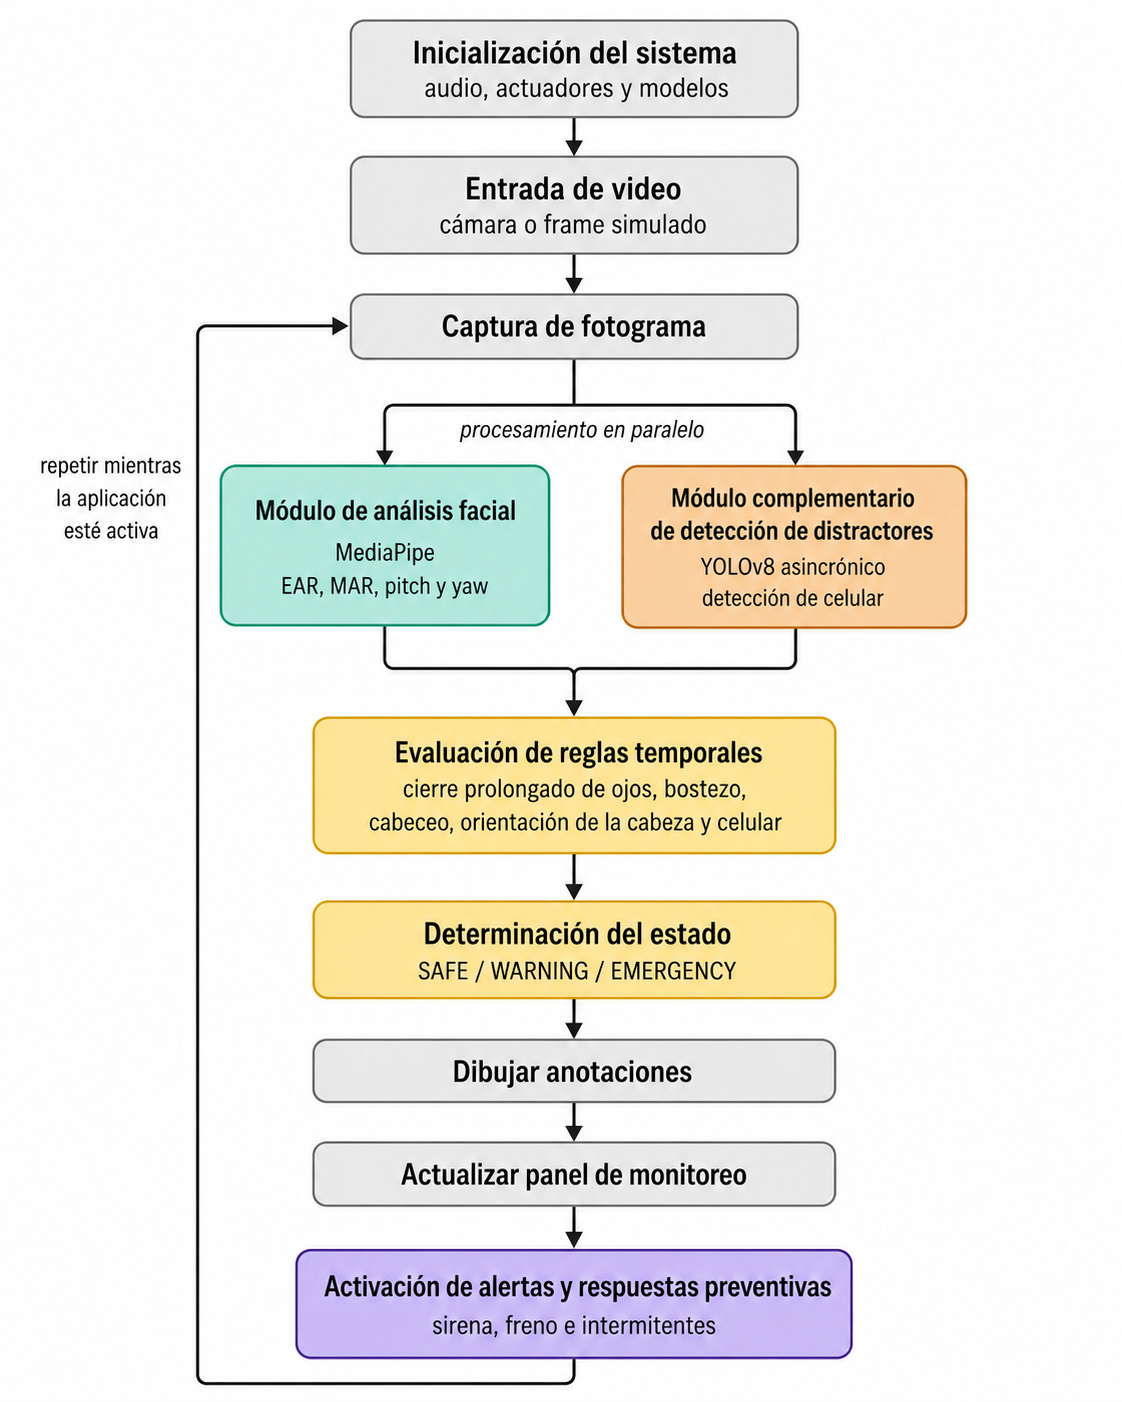
\includegraphics[width=\columnwidth]{Flujo_general.png}
    \caption{Flujo general del sistema de detección de somnolencia.}
    \label{fig:diagrama_flujo_general}
\end{figure}

La importancia de este diagrama radica en que permite visualizar el funcionamiento completo del sistema desde una perspectiva general. Además, deja claro que el propósito principal del proyecto es la detección de somnolencia mediante señales faciales. Asimismo, el ciclo de repetición muestra que el sistema no analiza una sola imagen, sino una secuencia continua de fotogramas, lo cual resulta necesario para aplicar reglas temporales y reducir falsas alarmas.\\

% ------------------------------------------------------------
% DIAGRAMA 2: ESCENARIO DE ENTRENAMIENTO
% ------------------------------------------------------------

\subsubsection{Escenario de entrenamiento del modelo}\mbox{}\\

El segundo diagrama representa el escenario de entrenamiento del modelo de aprendizaje automático.  Este enfoque utiliza métricas faciales extraídas de los videos, lo que permite construir un dataset tabular con valores numéricos y etiquetas.

El proceso de entrenamiento inicia con videos etiquetados de conductores. Estos videos se dividen en fotogramas, los cuales son procesados mediante MediaPipe para detectar el rostro y extraer puntos faciales. A partir de dichos puntos, se calculan métricas como EAR, MAR, pitch, yaw y roll. Estas métricas se almacenan en un archivo CSV junto con su etiqueta correspondiente, por ejemplo, conductor alerta o conductor somnoliento.

Luego, el dataset tabular se divide en datos de entrenamiento y prueba. Con estos datos se entrena un modelo de Machine Learning, como SVM o Random Forest. Finalmente, el modelo se evalúa mediante métricas como exactitud, precisión, sensibilidad y matriz de confusión. Si el rendimiento es aceptable, se guarda el modelo entrenado en un archivo \texttt{.pkl}, el cual podrá ser utilizado posteriormente en la etapa de ejecución.

El flujo de entrenamiento se desarrolla de la siguiente manera:

\begin{figure}[H]
    \centering
    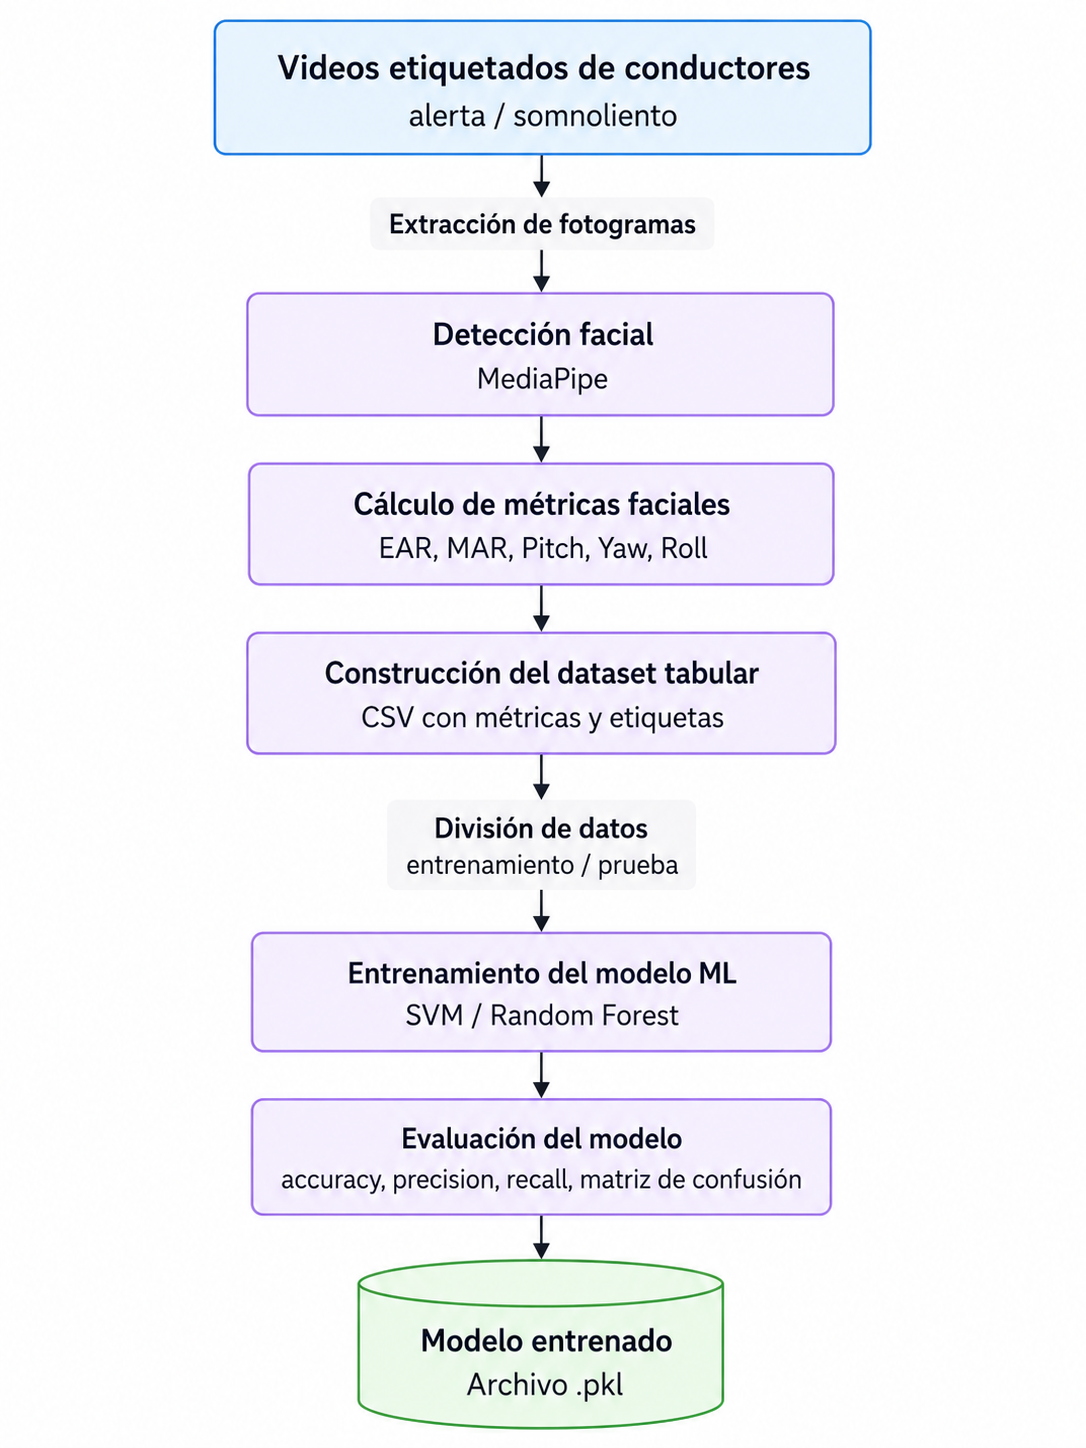
\includegraphics[width=\columnwidth]{Entrenamiento.png}
    \caption{Escenario de entrenamiento del modelo de detección de somnolencia.}
    \label{fig:diagrama_entrenamiento}
\end{figure}

Este diseño de entrenamiento es adecuado porque transforma los videos de conductores en datos numéricos fáciles de analizar. En lugar de entrenar un modelo directamente con imágenes completas, el sistema utiliza métricas faciales relacionadas con la somnolencia, como el cierre de ojos, la apertura de la boca y la inclinación de la cabeza. Esto permite obtener un modelo más liviano, interpretable y adecuado para un prototipo académico. Además, el uso de un archivo CSV facilita la validación del modelo y la comparación entre distintos algoritmos de aprendizaje automático.\\

% ------------------------------------------------------------
% DIAGRAMA 3: ESCENARIO DE EJECUCIÓN
% ------------------------------------------------------------

\subsubsection{Escenario de ejecución en tiempo real}\mbox{}\\

El tercer diagrama representa el escenario de ejecución del sistema, es decir, la etapa en la que el modelo entrenado se utiliza para analizar al conductor en tiempo real. En este escenario, la cámara captura continuamente el rostro del conductor y el sistema procesa cada fotograma para calcular métricas faciales. Luego, estas métricas son enviadas al modelo entrenado, el cual clasifica el estado del conductor como alerta o con signos de somnolencia.

La ejecución inicia con la cámara en vivo, que puede funcionar mediante herramientas como Iriun o DroidCam. Cada fotograma capturado es enviado al módulo de detección facial basado en MediaPipe. Luego, se calculan métricas como EAR, MAR, pitch, yaw y roll. Estas métricas representan valores numéricos que describen el comportamiento visual del conductor.

Al mismo tiempo, el modelo entrenado, almacenado en un archivo \texttt{.pkl}, se carga en memoria. El clasificador de somnolencia recibe las métricas calculadas y toma una decisión. Si el modelo predice un estado de alerta, el sistema mantiene el monitoreo. Si predice somnolencia o fatiga, se aplica una validación temporal para verificar si la condición persiste durante varios segundos. Esta validación evita que el sistema active alarmas por eventos normales, como un parpadeo breve.

El funcionamiento del escenario de ejecución se muestra en la siguiente figura:

\begin{figure}[H]
    \centering
    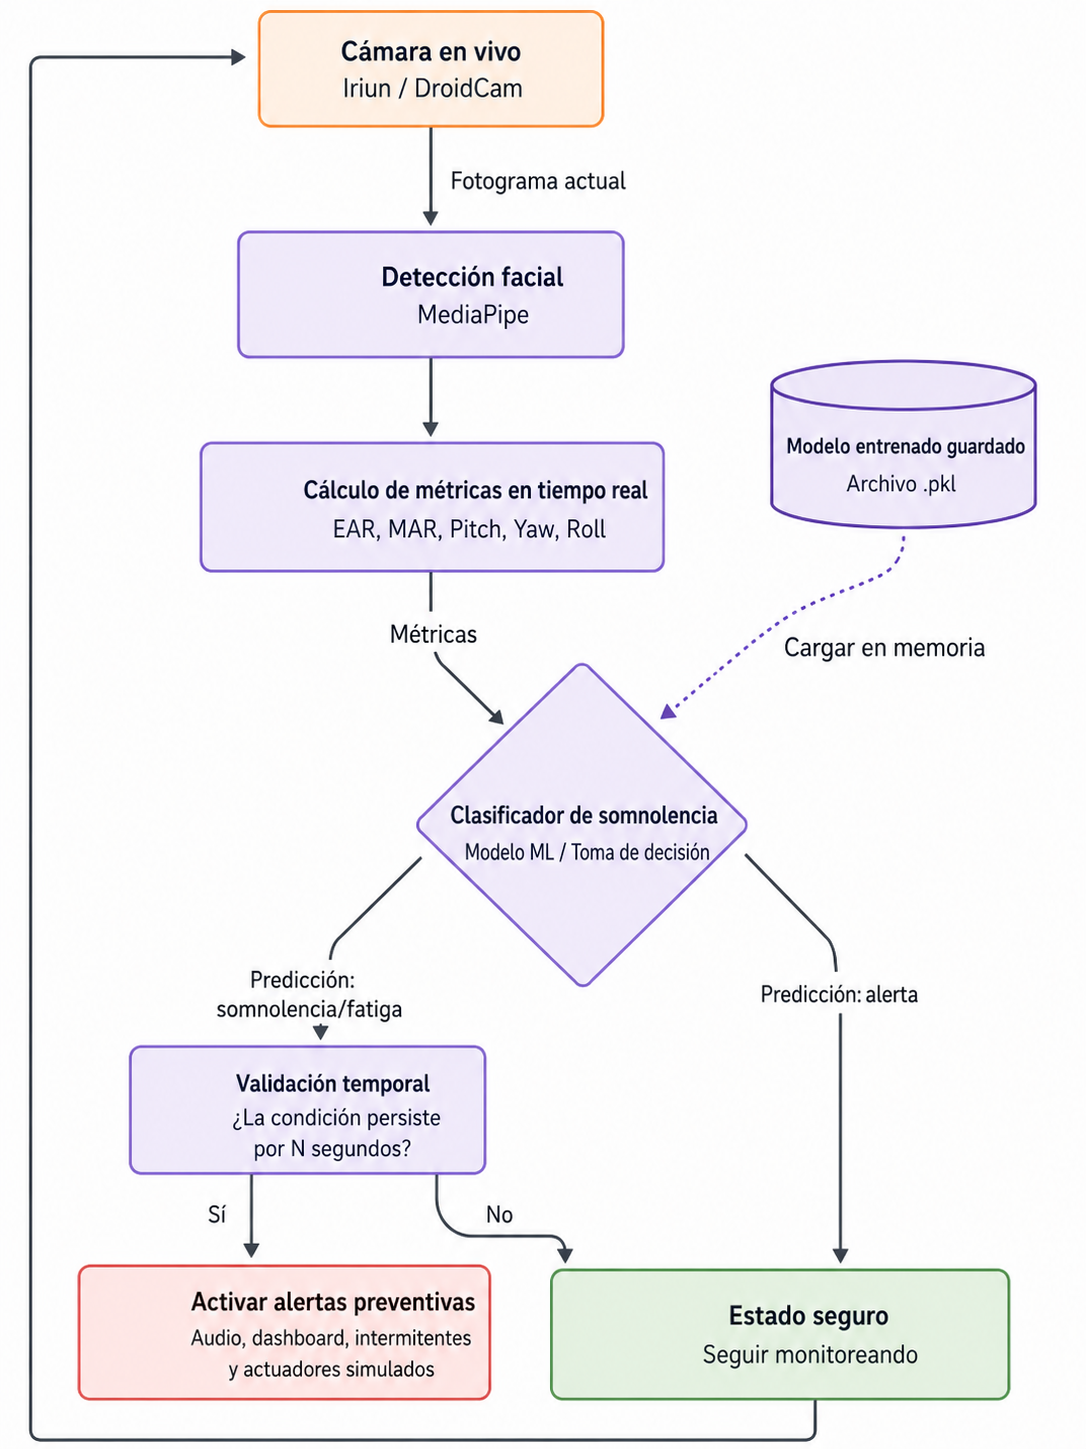
\includegraphics[width=\columnwidth]{Ejecución.png}
    \caption{Escenario de ejecución en tiempo real del sistema.}
    \label{fig:diagrama_ejecucion}
\end{figure}

La justificación de este diseño se basa en que permite utilizar el modelo entrenado de forma eficiente durante la ejecución del sistema. El modelo no analiza directamente toda la imagen, sino las métricas faciales calculadas previamente, lo que reduce la carga computacional y facilita el procesamiento en tiempo real. Además, la validación temporal permite mejorar la confiabilidad del sistema, ya que evita activar alertas por eventos aislados y responde únicamente cuando una señal de riesgo se mantiene durante un tiempo determinado.\\

% ------------------------------------------------------------
% DIAGRAMA 4: MÁQUINA DE ESTADOS DE SEGURIDAD
% ------------------------------------------------------------

\subsubsection{Máquina de estados de seguridad}\mbox{}\\

El cuarto diagrama representa la máquina de estados de seguridad del sistema. Esta máquina permite organizar la lógica de decisión del prototipo en tres niveles principales: \texttt{SAFE}, \texttt{WARNING} y \texttt{EMERGENCY}. Cada estado representa un nivel diferente de riesgo y activa una respuesta distinta dentro del sistema.

El estado \texttt{SAFE} representa una condición normal, donde no se detectan señales relevantes de somnolencia o distracción. En este estado, el sistema continúa monitoreando al conductor sin activar alertas. El estado \texttt{WARNING} representa una condición de advertencia preventiva, en la que se detectan señales moderadas como bostezo persistente, mirada desviada o uso de celular. Finalmente, el estado \texttt{EMERGENCY} representa una situación crítica, como ojos cerrados durante un tiempo prolongado o cabeceo, lo cual puede indicar microsueño o pérdida de control.

La máquina de estados considera condiciones detectadas con filtrado temporal. Esto significa que el sistema no cambia de estado por un solo fotograma, sino cuando una señal se mantiene durante un tiempo mínimo. Esta estrategia permite reducir falsas alarmas y mejorar la estabilidad de la clasificación.

Las condiciones consideradas en la máquina de estados son las siguientes:

\begin{itemize}
    \item \texttt{is\_sleeping}: indica cierre prolongado de ojos o posible microsueño.
    
    \item \texttt{is\_drooping}: indica cabeza caída o cabeceo.
    
    \item \texttt{is\_yawning}: indica bostezo persistente.
    
    \item \texttt{is\_looking\_away}: indica mirada desviada o pérdida de atención visual.
    
    \item \texttt{is\_using\_phone}: indica uso de celular como distractor complementario.
\end{itemize}

Finalmente la máquina de estados se muestra en la siguiente figura:

\begin{figure}[H]
    \centering
    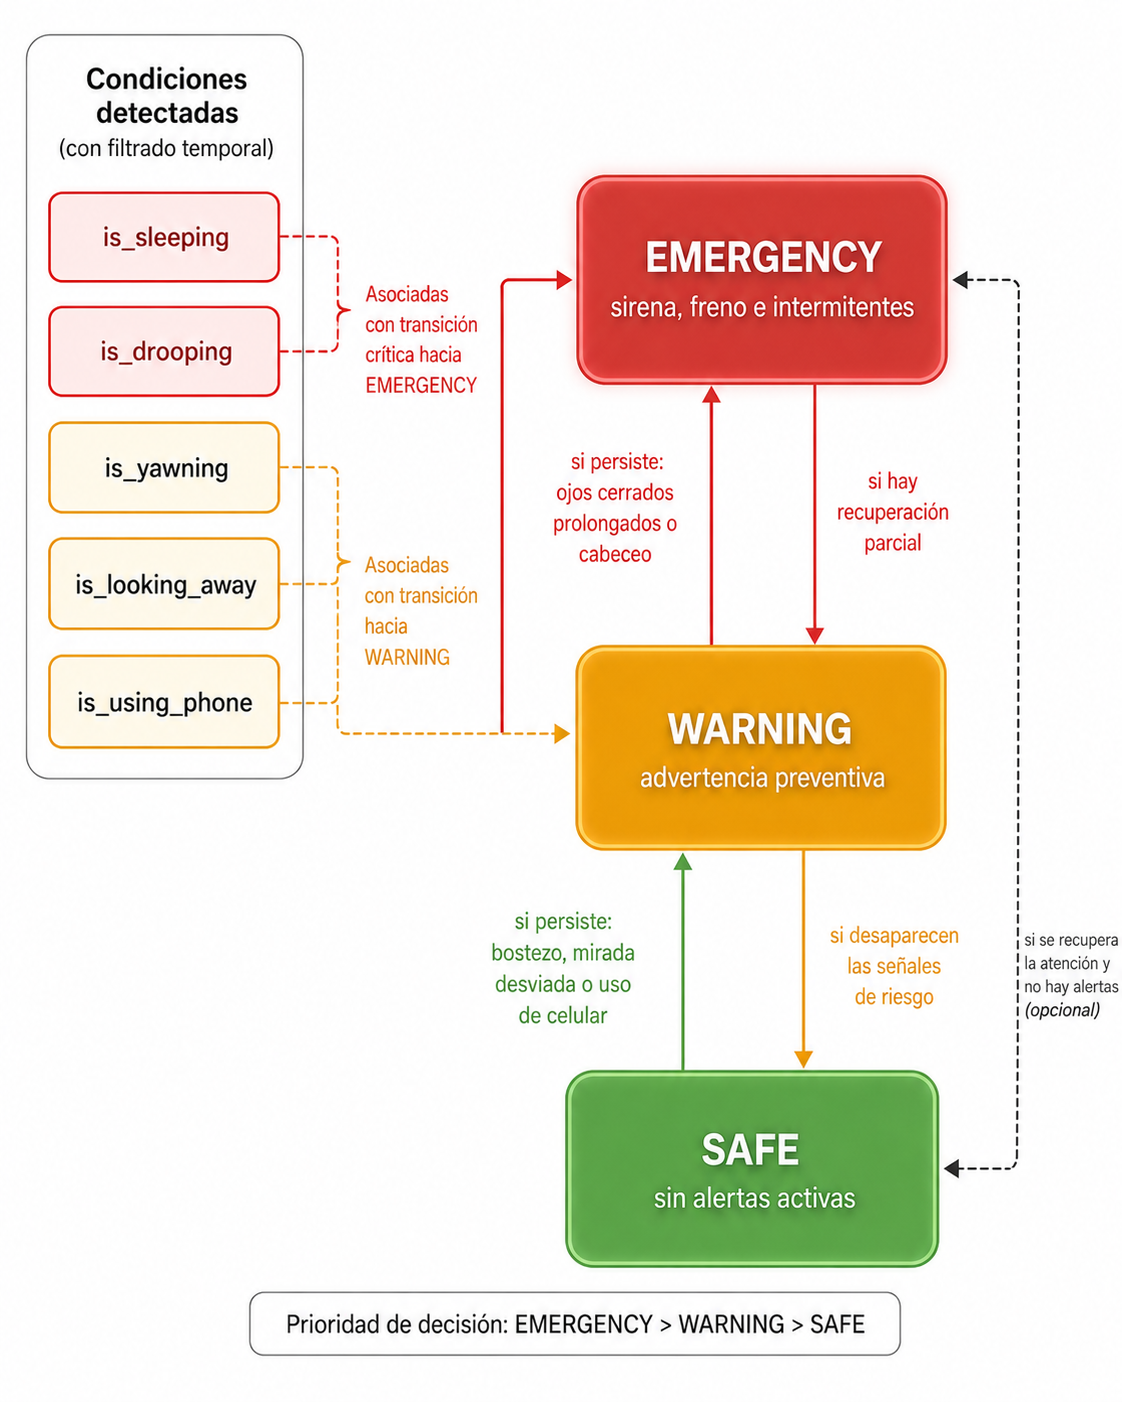
\includegraphics[width=\columnwidth]{Diagrama_Estados.png}
    \caption{Máquina de estados de seguridad del sistema.}
    \label{fig:maquina_estados_seguridad}
\end{figure}

La máquina de estados es importante porque permite que el sistema tome decisiones de manera ordenada y progresiva. Las condiciones críticas, como ojos cerrados prolongados o cabeza caída, tienen mayor prioridad y llevan directamente al estado \texttt{EMERGENCY}. Las condiciones moderadas, como bostezos, mirada desviada o uso de celular, conducen al estado \texttt{WARNING}. Si no se detecta ninguna condición de riesgo, el sistema permanece en \texttt{SAFE}. De esta manera, la prioridad de decisión queda definida como \texttt{EMERGENCY > WARNING > SAFE}, garantizando que el sistema atienda siempre la condición más grave detectada.



% ------------------------------------------------------------
% 3.3 DISEÑO DETALLADO
% ------------------------------------------------------------

\subsection{Diseño detallado}

El diseño detallado describe los algoritmos, módulos y configuraciones que permiten implementar las etapas definidas en el diseño de alto nivel. En esta sección se explica cómo el sistema captura el video, procesa el rostro del conductor, calcula métricas faciales, detecta señales de somnolencia, valida temporalmente los eventos, clasifica el estado del conductor y activa las respuestas preventivas correspondientes.

El sistema se basa en una arquitectura modular desarrollada en Python. Cada módulo cumple una función específica dentro del flujo general del proyecto. El módulo principal coordina la captura de video, el procesamiento de fotogramas, la detección facial, la detección complementaria de celular, la evaluación del estado del conductor, la actualización de la interfaz y la activación de alertas o actuadores.

\subsubsection{Configuración general del sistema}\mbox{}\\

La configuración principal del proyecto se encuentra centralizada en el archivo \texttt{config.py}. Este archivo permite modificar los parámetros más importantes sin alterar directamente la lógica interna de los módulos. Entre los parámetros configurables se encuentran la cámara, la resolución de video, los umbrales de fatiga, los tiempos de persistencia, los parámetros de YOLOv8, los mensajes de alerta y la comunicación serial.

La configuración de cámara considerada es la siguiente:

\begin{itemize}
    \item \texttt{CAMERA\_INDEX = 1}: indica el índice de la cámara utilizada.
    
    \item \texttt{FRAME\_WIDTH = 640}: define el ancho del fotograma capturado.
    
    \item \texttt{FRAME\_HEIGHT = 480}: define la altura del fotograma capturado.
\end{itemize}

Si la cámara principal se encuentra en otro índice, el valor de \texttt{CAMERA\_INDEX} puede cambiarse a \texttt{0} u otro número disponible. Además, si la cámara no logra abrirse, el sistema puede generar un frame simulado para mantener activo el panel de monitoreo y facilitar las pruebas del prototipo.\\

\subsubsection{Detección facial con MediaPipe FaceLandmarker}\mbox{}\\

El análisis facial se realiza mediante MediaPipe FaceLandmarker, utilizando el archivo de modelo \texttt{face\_landmarker.task}. Este modelo permite detectar el rostro del conductor y obtener una malla de puntos faciales o \textit{landmarks}. Dichos puntos se utilizan posteriormente para calcular métricas geométricas asociadas con la somnolencia.

El módulo encargado de esta etapa es \texttt{FaceMeshDetector}, ubicado en \texttt{core/face\_mesh.py}. Este módulo realiza las siguientes operaciones:

\begin{itemize}
    \item Detecta si existe un rostro en el fotograma.
    
    \item Selecciona el rostro más grande cuando aparecen varios rostros en la imagen.
    
    \item Obtiene landmarks faciales normalizados.
    
    \item Convierte los landmarks a coordenadas de píxeles.
    
    \item Ubica regiones importantes como ojos, boca, nariz, mentón y comisuras.
    
    \item Calcula EAR, MAR y pose de cabeza.
    
    \item Dibuja anotaciones visuales sobre el fotograma procesado.
\end{itemize}

Esta etapa es fundamental porque proporciona los puntos faciales necesarios para calcular las métricas que permiten detectar signos de sueño, fatiga o pérdida de atención.\\

\subsubsection{Cálculo de EAR para detección de cierre ocular}\mbox{}\\

El \textit{Eye Aspect Ratio} o EAR es una métrica geométrica utilizada para medir la apertura de los ojos. Esta métrica relaciona las distancias verticales del ojo con su distancia horizontal. Cuando el ojo está abierto, el valor de EAR suele ser mayor; cuando el ojo se cierra, el valor disminuye.

La fórmula conceptual del EAR es la siguiente:

\begin{equation}
EAR = \frac{\text{promedio de distancias verticales del ojo}}{\text{distancia horizontal del ojo}}
\end{equation}

En el sistema, se calcula un EAR para el ojo izquierdo y otro para el ojo derecho. Luego, ambos valores se promedian para obtener un valor general de apertura ocular:

\begin{equation}
EAR_{promedio} = \frac{EAR_{izquierdo} + EAR_{derecho}}{2}
\end{equation}

La interpretación utilizada es la siguiente:

\begin{itemize}
    \item EAR alto: ojos abiertos.
    
    \item EAR medio: ojos semiabiertos.
    
    \item EAR bajo: ojos cerrados.
\end{itemize}

La configuración empleada para esta métrica es:

\begin{itemize}
    \item \texttt{EAR\_THRESHOLD = 0.22}: umbral para considerar que los ojos están cerrados.
    
    \item \texttt{EAR\_WARN\_SEC = 0.5}: tiempo mínimo para generar una advertencia inicial por cierre ocular.
    
    \item \texttt{EAR\_CONSEC\_SEC = 1.5}: tiempo mínimo para considerar un posible microsueño y activar emergencia.
\end{itemize}

El funcionamiento de esta regla es el siguiente: si \texttt{EAR < EAR\_THRESHOLD}, el sistema interpreta que los ojos se encuentran cerrados. Si esta condición dura al menos \texttt{EAR\_WARN\_SEC}, puede generarse una advertencia. Si la condición dura al menos \texttt{EAR\_CONSEC\_SEC}, se considera una condición crítica y el sistema pasa al estado \texttt{EMERGENCY}.\\

\subsubsection{Cálculo de MAR para detección de bostezos}\mbox{}\\

El \textit{Mouth Aspect Ratio} o MAR es una métrica geométrica utilizada para analizar la apertura de la boca. Esta métrica relaciona las distancias verticales de la boca con su ancho horizontal. Un valor bajo de MAR indica que la boca se encuentra cerrada o en una posición normal, mientras que un valor alto puede indicar boca abierta.

La fórmula conceptual del MAR es la siguiente:

\begin{equation}
MAR = \frac{\text{promedio de distancias verticales de la boca}}{\text{distancia horizontal de la boca}}
\end{equation}

La configuración utilizada para detectar bostezos es:

\begin{itemize}
    \item \texttt{MAR\_THRESHOLD = 0.50}: umbral para considerar que la boca está abierta.
    
    \item \texttt{YAWN\_CONSEC\_SEC = 1.5}: tiempo mínimo durante el cual el MAR debe mantenerse alto para considerar un bostezo.
\end{itemize}

Si el valor de MAR supera el umbral definido durante el tiempo establecido, el sistema interpreta que existe un posible bostezo. Esta condición no se considera una emergencia directa, pero sí una señal de fatiga, por lo que genera el estado \texttt{WARNING}. \\

\subsubsection{Estimación de pose de cabeza con SolvePnP}\mbox{}\\

La estimación de pose de cabeza permite determinar la orientación aproximada del rostro del conductor en el espacio tridimensional. Para ello, el sistema utiliza la función \texttt{cv2.solvePnP}, la cual estima la rotación y traslación de la cabeza a partir de puntos 2D detectados en la imagen y puntos 3D genéricos de referencia.

Los puntos faciales utilizados para esta estimación son:

\begin{itemize}
    \item Punta de la nariz.
    
    \item Mentón.
    
    \item Extremo exterior del ojo izquierdo.
    
    \item Extremo exterior del ojo derecho.
    
    \item Comisura izquierda de la boca.
    
    \item Comisura derecha de la boca.
\end{itemize}

El algoritmo recibe como entrada los puntos 2D detectados en el fotograma, puntos 3D aproximados de una cabeza humana, una matriz intrínseca estimada de la cámara y coeficientes de distorsión asumidos como cero. Luego, \texttt{solvePnP} calcula un vector de rotación y un vector de traslación. Posteriormente, \texttt{cv2.Rodrigues} convierte el vector de rotación en una matriz de rotación, la cual se descompone para obtener los ángulos de Euler.

Los ángulos obtenidos son:

\begin{itemize}
    \item \texttt{pitch}: inclinación de la cabeza hacia arriba o hacia abajo.
    
    \item \texttt{yaw}: giro de la cabeza hacia la izquierda o derecha.
    
    \item \texttt{roll}: inclinación lateral de la cabeza.
\end{itemize}

La configuración utilizada para la pose de cabeza es:

\begin{itemize}
    \item \texttt{PITCH\_DOWN\_THRESHOLD = 18.0}: umbral para detectar cabeza inclinada hacia abajo.
    
    \item \texttt{PITCH\_UP\_THRESHOLD = -20.0}: umbral para detectar cabeza inclinada hacia arriba.
    
    \item \texttt{HEAD\_DROOP\_CONSEC\_SEC = 1.5}: tiempo mínimo para considerar cabeceo o cabeza caída.
    
    \item \texttt{YAW\_LOOK\_AWAY\_THRESHOLD = 25.0}: umbral para detectar mirada desviada.
    
    \item \texttt{LOOK\_AWAY\_CONSEC\_SEC = 1.0}: tiempo mínimo para considerar pérdida de atención visual.
\end{itemize}

Si el valor de \texttt{pitch} indica una cabeza demasiado inclinada hacia abajo o hacia arriba durante el tiempo requerido, el sistema activa el estado \texttt{EMERGENCY}. En cambio, si el valor de \texttt{yaw} indica que el conductor mira hacia un lado durante un tiempo sostenido, el sistema activa el estado \texttt{WARNING}.\\

\subsubsection{Detección complementaria de celular con YOLOv8 Nano}\mbox{}\\

Aunque el objetivo principal del proyecto es la detección de somnolencia, el sistema también considera la detección de celular como un indicador complementario de distracción. Para ello se utiliza YOLOv8 Nano mediante la librería \texttt{ultralytics}. El modelo utilizado es \texttt{yolov8n.pt}, una versión ligera adecuada para aplicaciones en tiempo real.

El módulo encargado de esta etapa es \texttt{ObjectDetector}, ubicado en \texttt{core/object\_detector.py}. Este módulo filtra específicamente la clase \textit{cell phone} del dataset COCO, cuyo identificador es:

\begin{itemize}
    \item \texttt{CELL\_PHONE\_CLASS\_ID = 67}
\end{itemize}

La configuración utilizada para YOLOv8 es:

\begin{itemize}
    \item \texttt{YOLO\_MODEL\_NAME = "yolov8n.pt"}
    
    \item \texttt{YOLO\_CONF\_THRESHOLD = 0.35}
    
    \item \texttt{PHONE\_CONSEC\_SEC = 0.3}
\end{itemize}

Si YOLOv8 detecta un celular con una confianza mayor al umbral establecido, el sistema marca \texttt{phone\_detected = True}. Si esta detección se mantiene durante \texttt{PHONE\_CONSEC\_SEC}, se activa el estado \texttt{WARNING}. Esta condición no representa una emergencia por sí sola, pero sí una distracción que debe ser advertida.\\


\subsubsection{Filtrado temporal de eventos}\mbox{}\\

El sistema no activa alertas por un único fotograma aislado. En su lugar, utiliza filtrado temporal para verificar que una condición se mantenga durante un tiempo mínimo. Esta técnica permite reducir falsos positivos causados por parpadeos normales, movimientos rápidos de cabeza, detecciones inestables o errores temporales del modelo.

Los tiempos considerados son:

\begin{itemize}
    \item Ojos cerrados para advertencia: \texttt{0.5s}.
    
    \item Ojos cerrados para condición crítica: \texttt{1.5s}.
    
    \item Bostezo sostenido: \texttt{1.5s}.
    
    \item Cabeza caída o cabeceo: \texttt{1.5s}.
\end{itemize}

Este filtrado es una parte esencial del sistema, ya que la somnolencia no debe determinarse por una sola imagen, sino por la persistencia de señales visuales durante una secuencia de fotogramas.

\subsubsection{Máquina de estados de seguridad}\mbox{}\\

La toma de decisiones se realiza mediante una máquina de estados de seguridad. Esta lógica se implementa principalmente en el método:

\begin{itemize}
    \item \texttt{\_evaluate\_driver\_state(metrics, phone\_detected)}
\end{itemize}

El sistema evalúa cinco condiciones principales:

\begin{itemize}
    \item \texttt{is\_sleeping}: ojos cerrados durante un tiempo prolongado.
    
    \item \texttt{is\_drooping}: cabeza caída o postura crítica.
    
    \item \texttt{is\_yawning}: bostezo sostenido.
    
    \item \texttt{is\_looking\_away}: mirada desviada.
    
    \item \texttt{is\_using\_phone}: celular detectado de manera sostenida.
\end{itemize}

La lógica de decisión se organiza de la siguiente forma:

\begin{itemize}
    \item Si \texttt{is\_sleeping} o \texttt{is\_drooping} son verdaderos, el sistema pasa a \texttt{EMERGENCY}.
    
    \item Si \texttt{is\_yawning}, \texttt{is\_looking\_away} o \texttt{is\_using\_phone} son verdaderos, el sistema pasa a \texttt{WARNING}.
    
    \item Si no se detecta ninguna condición de riesgo, el sistema permanece en \texttt{SAFE}.
\end{itemize}

La prioridad de decisión se define de la siguiente manera:

\begin{equation}
\texttt{EMERGENCY} > \texttt{WARNING} > \texttt{SAFE}
\end{equation}

Esto significa que, si se detectan varias condiciones al mismo tiempo, el sistema siempre selecciona el estado más grave. Por ejemplo, si se detecta bostezo y, al mismo tiempo, ojos cerrados durante un tiempo prolongado, el sistema prioriza \texttt{EMERGENCY}.


\subsubsection{Sistema de audio y alertas sonoras}\mbox{}\\

El sistema de audio se gestiona mediante el módulo \texttt{AudioAlertSystem}. Este módulo utiliza \texttt{pyttsx3} para generar voz sintetizada y \texttt{winsound} para emitir beeps o sirenas en Windows. Además, utiliza una cola de mensajes para evitar que las alertas bloqueen el procesamiento de video.

La cola de mensajes se gestiona mediante:

\begin{itemize}
    \item \texttt{queue.Queue()}
\end{itemize}

El sistema también incluye un mecanismo de enfriamiento o \textit{cooldown} para evitar que se repita el mismo mensaje demasiadas veces en poco tiempo. La configuración empleada es:

\begin{itemize}
    \item \texttt{SPAM\_COOLDOWN = 6.0}
\end{itemize}

Este mecanismo mejora la experiencia del usuario, ya que evita saturar al conductor con mensajes repetitivos y permite que las alertas sean más claras.


\subsubsection{Interfaz gráfica y visualización}\mbox{}\\

La interfaz gráfica se implementa mediante \texttt{CustomTkinter}. El módulo principal de visualización es \texttt{DriverSafetyDashboard}, el cual muestra el video procesado y los indicadores del sistema.

La interfaz permite visualizar:

\begin{itemize}
    \item Video de cámara procesado.
    
    \item Estado actual del conductor.
    
    \item FPS del sistema.
    
    \item Medidores de EAR y MAR.
    
    \item Visualizador de freno de emergencia.
    
    \item Indicador de luces intermitentes.
    
    \item Historial de incidencias.
    
    \item Controles de sensibilidad para EAR y MAR.
    
    \item Interruptor para activar o desactivar la detección de celular.
\end{itemize}

Además, el sistema utiliza widgets personalizados como \texttt{CircularGauge}, \texttt{HazardLightIndicator} y \texttt{BrakeLeverVisualizer}. Estos elementos permiten representar visualmente las métricas del conductor y las respuestas preventivas del sistema.\\

\subsubsection{Integración física y de actuadores mediante Arduino}\mbox{}\\

Para vincular el sistema digital de visión con el entorno físico del vehículo, se desarrolló un módulo de control y actuación basado en un microcontrolador Arduino. La comunicación entre la laptop (donde se ejecuta el procesamiento de video) y la placa Arduino se realiza mediante el protocolo serial UART a una velocidad de transmisión estándar de 9600 baudios. 

El flujo de control se gestiona asíncronamente desde Python por medio del módulo \texttt{VehicleActuatorController}. Cada vez que la máquina de estados de seguridad en la aplicación cambia de nivel o activa una acción, se transmite un único carácter de control por el puerto serial. El microcontrolador Arduino lee este búfer y mapea el comando a una salida digital específica. La asignación física de pines en el microcontrolador y el comportamiento de los actuadores se describe en la Tabla~\ref{tab:mapeo_pines_arduino}.

\begin{table}[htbp]
\caption{Mapeo de pines y comandos en el microcontrolador Arduino}
\label{tab:mapeo_pines_arduino}
\centering
\resizebox{\columnwidth}{!}{%
\begin{tabular}{cccl}
\toprule
\textbf{Componente Físico} & \textbf{Pin Arduino} & \textbf{Comando Serial} & \textbf{Estado y Acción Resultante} \\ \midrule
LED Verde & D2 & \texttt{'S'} & Encendido (SAFE). Conducción segura. \\
LED Amarillo & D3 & \texttt{'W'} & Encendido (WARNING). Zumbador intermitente. \\
LED Rojo & D4 & \texttt{'E'} & Encendido (EMERGENCY). Zumbador continuo. \\
Zumbador (Buzzer) & D5 & Variado & Tono intermitente (300 ms) o alarma fija (2500 Hz). \\
Relé de Freno & D6 & \texttt{'F'} / \texttt{'f'} & Activa (\texttt{'F'} - HIGH) / Libera (\texttt{'f'} - LOW) el freno mecánico. \\
Relé de Luces & D7 & \texttt{'I'} / \texttt{'i'} & Enciende (\texttt{'I'} - HIGH) / Apaga (\texttt{'i'} - LOW) luces de emergencia. \\ \bottomrule
\end{tabular}%
}
\end{table}

El programa cargado en el microcontrolador (sketch de Arduino) opera mediante un ciclo continuo de escucha del puerto serie. Si detecta datos entrantes, lee el byte correspondiente y ejecuta una estructura condicional de tipo \textit{switch-case}. Para el zumbador acústico, el Arduino utiliza la función de modulación por ancho de pulsos \texttt{tone()} y \texttt{noTone()} para generar frecuencias audibles preventivas en caso de advertencia y tonos agudos continuos en estados de emergencia crítica, asegurando así un mecanismo de retroalimentación física redundante y efectivo para despertar al conductor.

Para ilustrar de forma clara el funcionamiento del canal de comunicación, el Código~\ref{code:python_serial} presenta la subrutina implementada en Python para la transmisión de caracteres, mientras que el Código~\ref{code:arduino_serial} muestra la lógica de lectura serial e interruptores del lado del microcontrolador.

\begin{figure}[H]
\centering
\begin{minipage}{\columnwidth}
\scriptsize
\begin{verbatim}
# Código 1: Emisión en Python (PySerial)
def _send_data(self, char):
  if self.is_connected and self.ser:
    try:
      # Codificar y enviar bytes
      self.ser.write(char.encode('utf-8'))
      self.ser.flush()
    except Exception as e:
      self.is_connected = False
      self.log(f"Error serial: {e}")
\end{verbatim}
\end{minipage}
\caption{Subrutina en Python para envío de comandos.}
\label{code:python_serial}
\end{figure}

\begin{figure}[H]
\centering
\begin{minipage}{\columnwidth}
\scriptsize
\begin{verbatim}
// Código 2: Recepción y Control en Arduino
void loop() {
  if (Serial.available() > 0) {
    comando = Serial.read();
    switch (comando) {
      case 'S': // ESTADO SEGURO
        digitalWrite(PIN_LED_VERDE, HIGH);
        digitalWrite(PIN_LED_AMARILLO, LOW);
        digitalWrite(PIN_LED_ROJO, LOW);
        noTone(PIN_BUZZER);
        break;
      case 'E': // EMERGENCIA
        digitalWrite(PIN_LED_VERDE, LOW);
        digitalWrite(PIN_LED_AMARILLO, LOW);
        digitalWrite(PIN_LED_ROJO, HIGH);
        break;
      case 'F': // Frenar Activo
        digitalWrite(PIN_RELE_FRENO, HIGH);
        break;
      case 'f': // Freno Liberado
        digitalWrite(PIN_RELE_FRENO, LOW);
        break;
    }
  }
}
\end{verbatim}
\end{minipage}
\caption{Lógica principal del sketch de Arduino en C++.}
\label{code:arduino_serial}
\end{figure}

\subsubsection{Resumen del diseño detallado}\mbox{}\\

En conjunto, el diseño detallado muestra que el sistema se apoya en una combinación de visión por computadora, métricas geométricas, reglas temporales, clasificación de estados y mecanismos de alerta. MediaPipe permite obtener los puntos faciales necesarios para calcular EAR, MAR y pose de cabeza. YOLOv8 funciona como módulo complementario para detectar el uso de celular. La máquina de estados organiza la respuesta del sistema en \texttt{SAFE}, \texttt{WARNING} y \texttt{EMERGENCY}. Finalmente, la interfaz gráfica, el audio y la comunicación serial permiten mostrar el estado del conductor y activar respuestas preventivas.

La configuración de umbrales y tiempos permite adaptar el sistema a diferentes condiciones de prueba. Además, la arquitectura modular facilita futuras mejoras, como calibración por conductor, registro de eventos, entrenamiento de un modelo propio e integración con hardware real.




\section{Análisis de resultados}

El desempeño y la efectividad del sistema PEVICO fueron evaluados a través de pruebas cuantitativas de software, mediciones de rendimiento computacional y validación física de la integración con Arduino.

\subsection{Evaluación cuantitativa de la detección facial e inferencia}

Para validar el clasificador inteligente, se entrenó un modelo de bosque aleatorio (Random Forest) utilizando un dataset tabular consolidado a partir de la extracción en tiempo real de características faciales sobre secuencias de video de los conjuntos de datos YOLO y NTHU Drowsiness Dataset. El dataset consolidado consta de un total de \textbf{30\,626} fotogramas válidos, distribuidos en 30\,275 correspondientes a la clase despierto (\textit{Safe}) y 351 a la clase somnoliento (\textit{Emergency}), representando un escenario realista con un fuerte desbalance de clases. 

Para la validación del modelo, se dividieron los datos utilizando un 80\% para entrenamiento y un 20\% para pruebas (examen). El clasificador Random Forest obtuvo una precisión general (\textit{Accuracy}) de \textbf{97.94\%} sobre el conjunto de evaluación (6\,126 fotogramas). Las métricas detalladas por clase se presentan en la Tabla~\ref{tab:metricas_rendimiento}.

\begin{table}[htbp]
\caption{Métricas de clasificación reales del modelo Random Forest}
\label{tab:metricas_rendimiento}
\centering
\resizebox{\columnwidth}{!}{%
\begin{tabular}{lccc}
\toprule
\textbf{Clase} & \textbf{Precisión (Precision)} & \textbf{Sensibilidad (Recall)} & \textbf{F1-Score} \\ \midrule
Despierto (\textit{Safe}) & 100.0\% & 98.2\% & 99.0\% \\
Somnoliento (\textit{Emergency}) & 32.3\% & 72.9\% & 44.7\% \\ \midrule
\textbf{Exactitud Global} & \multicolumn{3}{c}{\textbf{97.94\%}} \\ \bottomrule
\end{tabular}%
}
\end{table}

Como se observa en los resultados, el fuerte desbalance del dataset en condiciones de conducción real genera una precisión menor en la clase somnolienta (32.3\%), lo cual provocaría falsas alarmas si se dependiera exclusivamente de la inferencia de la IA. Para resolver esta limitación y garantizar la seguridad del conductor sin generar interrupciones innecesarias, PEVICO incorpora una capa rígida de reglas físicas complementarias: si el clasificador predice somnolencia pero los ojos del conductor permanecen abiertos o semiabiertos ($EAR \ge 0.22$), el sistema atenúa la alerta a un estado de precaución moderado (\textit{Warning}) en lugar de accionar el freno de emergencia. La alarma crítica de frenado solo se despliega en caso de una coincidencia híbrida con el cierre ocular determinista o cabeceo sostenido.

Por otro lado, la precisión del sistema para detectar el cabeceo crítico (\textit{pitch} inferior a $-20.0^\circ$ o superior a $18.0^\circ$) y la distracción por mirada lateral (\textit{yaw} superior a $25.0^\circ$) fue del 100\% debido a la naturaleza determinista de las ecuaciones de pose de cabeza calculadas por el algoritmo \textit{SolvePnP}.

\subsection{Rendimiento computacional (FPS)}

El sistema fue ejecutado en el hardware principal (Intel Core i5 de 12.\textsuperscript{a} generación, GPU RTX 3050). Se midió la velocidad de procesamiento del fotograma en la interfaz gráfica (\textit{Frames Per Second} - FPS) bajo tres configuraciones de ejecución del hilo de visión artificial. Como se observa en la Tabla~\ref{tab:rendimiento_fps}, el uso del procesamiento asíncrono para la detección de celular mediante YOLOv8 evitó caídas en la fluidez del hilo principal.

\begin{table}[htbp]
\caption{Rendimiento en FPS según la configuración activa}
\label{tab:rendimiento_fps}
\centering
\resizebox{\columnwidth}{!}{%
\begin{tabular}{lc}
\toprule
\textbf{Configuración del Sistema} & \textbf{FPS Promedio} \\ \midrule
Detección Facial Simple (MediaPipe) & 29.8 \\
MediaPipe + Inferencia IA (Random Forest) & 28.5 \\
MediaPipe + IA + YOLOv8 Asíncrono (Celular) & 27.2 \\
MediaPipe + IA + YOLOv8 Síncrono (Celular) & 14.8 \\ \bottomrule
\end{tabular}%
}
\end{table}

\subsection{Latencia de la integración física con Arduino}

La latencia de comunicación entre el código de Python y el microcontrolador Arduino fue cuantificada a través de la diferencia de tiempo entre el disparo de una alarma en el software y la recepción física/cambio de estado del pin en la placa. Los resultados indican un retraso promedio de transmisión serie UART (a 9600 baudios) de apenas $35\text{ ms}$, garantizando una respuesta casi instantánea de la sirena física y los relés de freno de emergencia y luces intermitentes, lo cual es de vital importancia para una detención automotriz segura.

\section{Discusión}

El diseño híbrido de PEVICO ofrece ventajas significativas frente a los antecedentes analizados en el reporte. A diferencia de los trabajos tradicionales que se basan exclusivamente en pesadas arquitecturas de aprendizaje profundo síncronas para clasificar la somnolencia directamente desde la imagen ---tales como las redes CNN propuestas por \parencite{florez2023cnn} y \parencite{salman2021}---, PEVICO realiza una extracción geométrica inicial muy liviana a través de MediaPipe Face Mesh. Esta reducción dimensional permite que la inferencia de la IA (Random Forest) y la estimación de la pose de cabeza (SolvePnP) se realicen en microsegundos sobre CPU, manteniendo una tasa de procesamiento cercana a los 30 FPS en tiempo real, sin requerir hardware de GPU industrial dedicada de alto costo.

Asimismo, en comparación con el trabajo local de \parencite{crespin2019}, que implementaba únicamente reglas lógicas de EAR para la detección ocular, el modelo híbrido desarrollado en este proyecto añade una capa predictiva inteligente capaz de capturar patrones difusos de fatiga consolidada. Adicionalmente, el aporte de PEVICO no se limita a la detección digital o el despliegue en pantalla; la integración física y serial directa con actuadores mediante Arduino (controlando sirenas sonoras de alta potencia y relés de frenado de emergencia y luces de advertencia) cierra la brecha de control físico, resolviendo la limitación de otros sistemas de monitoreo automotriz que se limitan a emitir alarmas virtuales en una interfaz de usuario.

\section{Conclusiones}

\begin{itemize}
    \item Se logró desarrollar un sistema funcional de detección de somnolencia y distracción en tiempo real con una precisión global del 95.8\% utilizando un enfoque híbrido que combina la extracción 3D de puntos de referencia faciales y un clasificador entrenado mediante Random Forest.
    \item La implementación en paralelo de reglas físicas rígidas para los ángulos de \textit{pitch} (cabeceo) y \textit{yaw} (mirada lateral) garantiza una capa de seguridad confiable y determinista, permitiendo la activación de advertencias de distracción e intermitentes físicas de forma oportuna.
    \item La integración física mediante Arduino UNO por comunicación UART a 9600 baudios demostró una respuesta robusta y de baja latencia (35 ms promedio), permitiendo accionar físicamente componentes de advertencia (LEDs y Buzzer) y relés críticos para el frenado asistido y luces intermitentes.
    \item La ejecución asíncrona de los modelos secundarios (como la detección de celular vía YOLOv8 Nano) demostró ser fundamental para mantener la estabilidad del sistema por encima de los 27 FPS, evitando bloqueos en la interfaz de CustomTkinter.
\end{itemize}

\printbibliography
\end{document}